\subsection{Composition product and connecting homomorphisms of extension modules}

PROPOSITION 5. — Let

\[
0 \to {\bf M} ^ {\prime} \stackrel {f} {\to} {\bf M} \stackrel {g} {\to} {\bf M} ^ {\prime \prime} \to 0\tag{8}
\]

be an exact sequence of left A-modules, \(\theta\in\mathrm{Ext}_{\mathbf{A}}^{1}\left(\mathbf{M}^{\prime\prime},\mathbf{M}^{\prime}\right)\) the associated class, N a left A-module, n an integer.

\begin{enumerate}
\def\labelenumi{\alph{enumi})}
\item
  The connecting homomorphism \(\delta^{n}(\mathbf{N},\mathcal{E}):\operatorname{Ext}_{\mathbf{A}}^{n}(\mathbf{N},\mathbf{M}^{\prime \prime})\to \operatorname{Ext}_{\mathbf{A}}^{n + 1}(\mathbf{N},\mathbf{M}^{\prime})\) is the composition product \(\alpha \mapsto \theta \circ \alpha\) by \(\theta\) .
\item
  The connecting homomorphism \(\delta^{n}(\mathcal{E},\mathbf{N}):\operatorname{Ext}_{\mathbf{A}}^{n}(\mathbf{M}^{\prime},\mathbf{N})\to\operatorname{Ext}_{\mathbf{A}}^{n+1}(\mathbf{M}^{\prime\prime},\mathbf{N})\) is the composition product \(\alpha\mapsto(-1)^{n+1}\alpha\circ\theta\) by \((-1)^{n+1}\theta\) .
\item
  Consider a commutative diagram
\end{enumerate}

\[
\begin{array}{l} 0 \xrightarrow {} \mathrm{M} ^ {\prime} \xrightarrow {f} \mathrm{M} \xrightarrow {g} \mathrm{M} ^ {\prime \prime} \xrightarrow {} 0 \\ 0 \xrightarrow {} \mathrm{M} ^ {\prime} \xrightarrow {e _ {\mathrm{M} ^ {\prime}}} \mathrm{I} ^ {0} (\mathrm{M} ^ {\prime}) \xrightarrow {\delta^ {0}} \mathrm{I} ^ {1} (\mathrm{M} ^ {\prime}). \end{array}
\]

By definition, \(\theta\) is the class of \(-v^{1}\in\mathrm{Homgr}_{\mathbf{A}}^{1}(\mathbf{M}^{\prime\prime},\mathbf{I}(\mathbf{M}^{\prime}))\) . Let moreover \(\alpha\in\mathrm{Ext}_{\mathbf{A}}^{n}(\mathbf{N},\mathbf{M}^{\prime\prime})\) , represented by an element \(a\) of \(\mathrm{Homgr}_{\mathbf{A}}^{n}(\mathbf{L}(\mathbf{N}),\mathbf{M}^{\prime\prime})\) . By construction, \(\delta^{n}(\alpha)\) is obtained as follows: one lifts \(a^{n}\in\mathrm{Hom}_{\mathbf{A}}(\mathbf{L}_{n}(\mathbf{N}),\mathbf{M}^{\prime\prime})\) to

\[
b \in \operatorname{Hom} _ {\mathbf {A}} \left(\mathrm{L} _ {n} (\mathrm{N}), \mathrm{M}\right),
\]

and \(\delta^n (\alpha)\) is the class of \(e_{\mathbf{M}'}\circ c\) where \(c\in \mathrm{Hom}_{\mathbf{A}}\left(\mathbf{L}_{n + 1}(\mathbf{N}),\mathbf{M}'\right)\) is such that

\[
f \circ c = \mathrm{D} b = (- 1) ^ {n + 1} b \circ d _ {n + 1}.
\]

We thus have a commutative diagram

\[
\begin{array}{c} L _ {n + 1} (N) \xrightarrow {d _ {n + 1}} L _ {n} (N) \\ (- 1) ^ {n + 1} c \Big \downarrow \\ 0 \longrightarrow M ^ {\prime} \xrightarrow {f} M \xrightarrow {g} M ^ {\prime \prime} \longrightarrow 0 \\ 1 _ {M ^ {\prime}} \Big \downarrow \\ 0 \longrightarrow M ^ {\prime} \xrightarrow {e _ {M ^ {\prime}}} I ^ {0} (M ^ {\prime}) \xrightarrow {\delta^ {0}} I ^ {1} (M ^ {\prime}). \end{array}
\]

But, in \(\operatorname{Homgr}_{\mathbf{A}}(\mathbf{L}(\mathbf{N}), \mathbf{l}(\mathbf{M}'))\) , we have

\[
\mathrm{D} \left(v ^ {0} \circ b\right) = \delta^ {0} \circ v ^ {0} \circ b - (- 1) ^ {n} v ^ {0} \circ b \circ d _ {n + 1} = v ^ {1} \circ a ^ {n} + e _ {\mathrm{M} ^ {\prime}} \circ c.
\]

The classes of \(e_{\mathbf{M}'} \circ c\) and \((-v^1) \circ a\) in \(\operatorname{Ext}_{\mathbf{A}}^{n+1}(\mathbf{N}, \mathbf{M}')\) are equal, whence \(a\) ).

\begin{enumerate}
\def\labelenumi{\alph{enumi})}
\setcounter{enumi}{1}
\tightlist
\item
  Consider a commutative diagram
\end{enumerate}

\[
\begin{array}{c} \mathrm{L} _ {1} (\mathrm{M} ^ {\prime \prime}) \xrightarrow {d _ {1}} \mathrm{L} _ {0} (\mathrm{M} ^ {\prime \prime}) \xrightarrow {p _ {\mathrm{M} ^ {\prime \prime}}} \mathrm{M} ^ {\prime \prime} \longrightarrow 0 \\ \Biggl \downarrow u _ {1} \\ 0 \longrightarrow \mathrm{M} ^ {\prime} \xrightarrow {f} \mathrm{M} \xrightarrow {g} \mathrm{M} ^ {\prime \prime} \longrightarrow 0. \end{array}
\]

By definition, \(\theta\) is the class of \(-u_{1}\in\mathrm{Homgr}_{\mathbf{A}}^{1}(\mathrm{L}(\mathbf{M}^{\prime\prime}),\mathbf{M}^{\prime})\) . Let moreover \(\alpha\in\mathrm{Ext}^{n}(\mathbf{M}^{\prime},\mathbf{N})\) represented by an element \(a\) of \(\mathrm{Homgr}_{\mathbf{A}}^{n}(\mathbf{M}^{\prime},\mathrm{I}(\mathbf{N}))\) . By construction, \(\delta^{n}(\alpha)\) is obtained as follows: one extends \(a^{n}\in\mathrm{Hom}_{\mathbf{A}}(\mathbf{M}^{\prime},\mathrm{I}^{n}(\mathbf{N}))\) to

\[
b \in \operatorname{Hom} _ {\mathbf {A}} (\mathbf {M}, \mathrm{I} ^ {n} (\mathbf {N}))
\]

and \(\delta^n (\alpha)\) is the class of \(c\circ p_{\mathbf{M}''}\) , where \(c\in \mathrm{Hom}_{\mathbf{A}}(\mathbf{M}^{\prime \prime},\mathrm{I}^{n + 1}(\mathbf{N}))\) is such that

\[
g \circ c = D b = \delta^ {n + 1} \circ b.
\]

We thus have a commutative diagram

\[
\begin{array}{c} L _ {1} (M ^ {\prime \prime}) \xrightarrow {d _ {1}} L _ {0} (M ^ {\prime \prime}) \xrightarrow {p _ {M ^ {\prime \prime}}} M ^ {\prime \prime}. \longrightarrow 0 \\ u _ {1} \Biggl \downarrow \quad \quad \quad \quad \quad \quad \quad \quad \quad \quad \quad \quad \quad \quad \quad \quad \quad \quad \quad \quad \quad \quad \quad \quad \quad \quad \quad \quad \quad \quad \quad \quad \quad \quad \quad \quad \quad \quad \quad \quad \quad \quad \quad \quad \quad \quad \quad 1 _ {M ^ {\prime}} \\ 0 \longrightarrow M ^ {\prime} \xrightarrow {f} M \xrightarrow {g} M ^ {\prime \prime} \longrightarrow 0 \\ a ^ {n} \Biggl \downarrow \quad \quad \quad \quad \quad \quad \quad \quad \quad \quad \quad \quad c \Biggl \downarrow \\ I ^ {n} (N) \xrightarrow {\delta^ {n}} I ^ {n + 1} (N). \end{array}
\]

But, in \(\operatorname{Homgr}_{\mathbf{A}}(\mathbf{L}(\mathbf{M}^{\prime \prime}),\mathbf{l}(\mathbf{N}))\) , we have

\[
\mathrm{D} (b \circ u _ {0}) = \delta^ {n} \circ b \circ u _ {0} - (- 1) ^ {n} b \circ u _ {0} \circ c = c \circ p - (- 1) ^ {n} a ^ {n} \circ u _ {1}.
\]

The classes of \(c \circ p\) and of \((-1)^{n+1} a^n \circ (-u_1)\) in \(\operatorname{Ext}_{\mathbf{A}}^{n+1} (\mathbf{M}''\) , \(\mathbf{N}\) ) are therefore equal, whence \(b\) ).

COROLLARY 1. --- a) The connecting homomorphism Hom \(_{A}\) (M'', M'') → Ext \(_{A}^{1}\) (M'', M') sends 1 \(_{M''}\) to θ.

\begin{enumerate}
\def\labelenumi{\alph{enumi})}
\setcounter{enumi}{1}
\tightlist
\item
  The connecting homomorphism \(\operatorname{Hom}_{\mathbf{A}}(\mathbf{M}^{\prime},\mathbf{M}^{\prime})\to\operatorname{Ext}_{\mathbf{A}}^{1}(\mathbf{M}^{\prime\prime},\mathbf{M}^{\prime})\) sends \(1_{M'}\) to \(-\theta\).
\end{enumerate}

COROLLARY 2. --- Consider two exact sequences of left A-modules

\[
0 \rightarrow \mathbf {M} ^ {\prime} \rightarrow \mathbf {M} \rightarrow \mathbf {M} ^ {\prime \prime} \rightarrow 0
\]

\[
0 \rightarrow \mathrm{N} ^ {\prime} \rightarrow \mathrm{N} \rightarrow \mathrm{N} ^ {\prime \prime} \rightarrow 0.
\]

Then the composed homomorphisms of connecting homomorphisms

\[
\operatorname{Ext} _ {\mathbf {A}} ^ {n} \left(\mathrm{M} ^ {\prime}, \mathrm{N} ^ {\prime \prime}\right)\rightarrow \operatorname{Ext} _ {\mathbf {A}} ^ {n + 1} \left(\mathrm{M} ^ {\prime \prime}, \mathrm{N} ^ {\prime \prime}\right)\rightarrow \operatorname{Ext} _ {\mathbf {A}} ^ {n + 2} \left(\mathrm{M} ^ {\prime \prime}, \mathrm{N} ^ {\prime}\right)
\]

and

\[
\operatorname{Ext} _ {\mathbf {A}} ^ {n} \left(\mathrm{M} ^ {\prime}, \mathrm{N} ^ {\prime \prime}\right)\rightarrow \operatorname{Ext} _ {\mathbf {A}} ^ {n + 1} \left(\mathrm{M} ^ {\prime}, \mathrm{N} ^ {\prime}\right)\rightarrow \operatorname{Ext} _ {\mathbf {A}} ^ {n + 2} \left(\mathrm{M} ^ {\prime \prime}, \mathrm{N} ^ {\prime}\right)
\]

are opposite.

Indeed, if \(\theta_{1}\) , \(\theta_{2}\) are the classes associated with the given exact sequences, and if \(\alpha \in \operatorname{Ext}_{\mathbf{A}}^{n}(\mathbf{M}', \mathbf{M}'')\) the images of \(\alpha\) are respectively

\[
\theta_ {2} \circ ((- 1) ^ {n + 1} \alpha \circ \theta_ {1}) \quad \text { and } \quad (\theta_ {2} \circ \alpha) \circ ((- 1) ^ {n + 2} \theta_ {1}).
\]

Consider an exact sequence of left A-modules

\[
0 \rightarrow \mathrm{N} \rightarrow \mathrm{R} _ {n} \xrightarrow {f _ {n}} \mathrm{R} _ {n - 1} \xrightarrow {f _ {n - 1}} \dots \rightarrow \mathrm{R} _ {1} \xrightarrow {f _ {1}} \mathrm{M} \rightarrow 0\tag{S}
\]

and set \(K_{0} = M\) , \(K_{i} = Ker f_{i}, i = 1, \ldots, n - 1\) , \(K_{n} = N\) . We therefore have exact sequences

\[
0 \to \mathbf {K} _ {i} \to \mathbf {R} _ {i} \to \mathbf {K} _ {i - 1} \to 0, \quad 1 \leqslant i \leqslant n,\tag{9}
\]

to which are associated, for every left A-module P, connecting homomorphisms

\[
\begin{array}{r l}&{\mathrm{Ext} _ {\mathbf {A}} ^ {m} \left(\mathrm{P}, \mathbf {K} _ {i - 1}\right)\rightarrow \mathrm{Ext} _ {\mathbf {A}} ^ {m + 1} \left(\mathrm{P}, \mathbf {K} _ {i}\right),}\\&{\qquad \mathrm{Ext} _ {\mathbf {A}} ^ {m} \left(\mathbf {K} _ {i}, \mathrm{P}\right)\rightarrow \mathrm{Ext} _ {\mathbf {A}} ^ {m + 1} \left(\mathbf {K} _ {i - 1}, \mathrm{P}\right),}\end{array}
\]

whence by composition of the iterated connecting homomorphisms, associated with (S)

\[
\begin{array}{l} \delta^ {m} (\mathrm{P}, \mathcal {S}): \operatorname{Ext} _ {\mathrm{A}} ^ {m} (\mathrm{P}, \mathrm{M}) \to \operatorname{Ext} _ {\mathrm{A}} ^ {m + n} (\mathrm{P}, \mathrm{N}) \\ \delta^ {m} (\mathcal {S}, \mathrm{P}): \operatorname{Ext} _ {\mathrm{A}} ^ {m} (\mathrm{N}, \mathrm{P}) \to \operatorname{Ext} _ {\mathrm{A}} ^ {m + n} (\mathrm{M}, \mathrm{P}). \end{array}
\]

COROLLARY 3. --- If \(\theta\in\mathrm{Ext}_{\mathbf{A}}^{n}(\mathbf{M},\mathbf{N})\) is the class of the exact sequence \((\mathcal{S})\) , we have

\[
\delta^ {m} (\mathrm{P}, \mathscr {S}) (\alpha) = \theta \circ \alpha , \quad \delta^ {m} (\mathscr {S}, \mathrm{P}) (\beta) = (- 1) ^ {m n + n (n + 1) / 2} \beta \circ \theta .
\]

If \(\theta_{i}\in\mathrm{Ext}_{\mathbf{A}}^{1}(\mathbf{K}_{i-1},\mathbf{K}_{i})\) is the class associated with the exact sequence (9), we have by prop. 5

\[
\begin{array}{l} \delta^ {m} (\mathrm{P}, \mathcal {S}) (\alpha) = \theta_ {n} \circ \dots \circ \theta_ {2} \circ \theta_ {1} \circ \alpha \\ \delta^ {m} (\mathcal {S}, \mathrm{P}) (\beta) = (- 1) ^ {(m + 1) + \dots + (m + n)} \beta \circ \theta_ {n} \circ \dots \circ \theta_ {1}. \end{array}
\]

Moreover, by prop. 3 (X, p.~118), we have \(\theta = \theta_{n} \circ \cdots \circ \theta_{1}\) . The corollary follows immediately from this, and from the relation (E, III, p.~44)

\[
(m + 1) + \dots + (m + n) = m n + n (n + 1) / 2.
\]

COROLLARY 4. --- If each module \(\mathbf{R}_i\) , \(i = 1, \ldots, n\) , is injective (resp. projective), the map \(\alpha \mapsto \theta \circ \alpha\) (resp. \(\alpha \mapsto \alpha \circ \theta\) ) from \(\operatorname{Ext}_{\mathbf{A}}^{m}(\mathbf{P}, \mathbf{M})\) to \(\operatorname{Ext}_{\mathbf{A}}^{m+n}(\mathbf{P}, \mathbf{N})\) (resp. from \(\operatorname{Ext}_{\mathbf{A}}^{m}(\mathbf{N}, \mathbf{P})\) to \(\operatorname{Ext}_{\mathbf{A}}^{m+n}(\mathbf{M}, \mathbf{P})\) ) is bijective for every A-module P and every integer \(m > 0\) . This follows indeed from cor. 3 and the exact sequences

\[
\operatorname{Ext} _ {\mathbf {A}} ^ {m + i - 1} \left(\mathrm{P}, \mathrm{R} _ {i}\right)\rightarrow \operatorname{Ext} _ {\mathbf {A}} ^ {m + i - 1} \left(\mathrm{P}, \mathrm{K} _ {i - 1}\right)\rightarrow \operatorname{Ext} _ {\mathbf {A}} ^ {m + i} \left(\mathrm{P}, \mathrm{K} _ {i}\right)\rightarrow \operatorname{Ext} _ {\mathbf {A}} ^ {m + i} \left(\mathrm{P}, \mathrm{R} _ {i}\right)
\]

\[
\left(\text { resp. } \operatorname{Ext} _ {\mathbf {A}} ^ {m + i - 1} \left(\mathrm{R} _ {i}, \mathrm{P}\right)\rightarrow \operatorname{Ext} _ {\mathbf {A}} ^ {m + i - 1} \left(\mathrm{K} _ {i}, \mathrm{P}\right)\rightarrow \operatorname{Ext} _ {\mathbf {A}} ^ {m + i} \left(\mathrm{K} _ {i - 1}, \mathrm{P}\right)\rightarrow \operatorname{Ext} _ {\mathbf {A}} ^ {m + i} \left(\mathrm{R} _ {i}, \mathrm{P}\right)\right),
\]

whose extreme terms are zero by hypothesis.

Remark. --- The definitions and propositions of nos. 3 to 6 apply to right A-modules, considered as left modules over the opposite ring A° of A.

\subsection{\texorpdfstring{The homomorphism \(\operatorname{Ext}_{\mathbf{A}}(\mathbf{P}, \mathbf{Q}) \otimes \operatorname{Tor}^{\mathbf{A}}(\mathbf{P}, \mathbf{M}) \to \operatorname{Tor}^{\mathbf{A}}(\mathbf{Q}, \mathbf{M})\)}{The homomorphism \textbackslash operatorname\{Ext\}\_\{\textbackslash mathbf\{A\}\}(\textbackslash mathbf\{P\}, \textbackslash mathbf\{Q\}) \textbackslash otimes \textbackslash operatorname\{Tor\}\^{}\{\textbackslash mathbf\{A\}\}(\textbackslash mathbf\{P\}, \textbackslash mathbf\{M\}) \textbackslash to \textbackslash operatorname\{Tor\}\^{}\{\textbackslash mathbf\{A\}\}(\textbackslash mathbf\{Q\}, \textbackslash mathbf\{M\})}}

Let M be a left A-module, and let P and Q be two right A-modules. Consider the homomorphism \(\operatorname{Homgr}_{\mathbf{A}}(\mathrm{L}(\mathrm{P}), \mathrm{L}(\mathrm{Q})) \otimes_{k} (\mathrm{L}(\mathrm{P}) \otimes_{\mathbf{A}} \mathrm{L}(\mathrm{M})) \to \mathrm{L}(\mathrm{Q}) \otimes_{\mathbf{A}} \mathrm{L}(\mathrm{M})\) which to \(f \otimes (x \otimes y)\) associates \(f(x) \otimes y\) . By X, p.~99, this is a morphism of complexes. From this one deduces a graded \(k\) -linear map of degree 0

\[
\mathrm{H} (\operatorname{Homgr} _ {\mathrm{A}} (\mathrm{L} (\mathrm{P}), \mathrm{L} (\mathrm{Q}))) \otimes_ {k} \operatorname{Tor} ^ {\mathrm{A}} (\mathrm{P}, \mathrm{M}) \rightarrow \operatorname{Tor} ^ {\mathrm{A}} (\mathrm{Q}, \mathrm{M})
\]

hence, via the isomorphism \(\varphi(\mathbf{L}(\mathbf{P}),\mathbf{L}(\mathbf{Q}))\) of § 6 (X, p.~100, th. 1), a graded \(k\) -linear map of degree 0

\[
\operatorname{Ext} _ {\mathbf {A}} (\mathrm{P}, \mathrm{Q}) \otimes_ {k} \operatorname{Tor} ^ {\mathbf {A}} (\mathrm{P}, \mathrm{M}) \rightarrow \operatorname{Tor} ^ {\mathbf {A}} (\mathrm{Q}, \mathrm{M}),\tag{10}
\]

corresponding to k-bilinear maps

\[
c _ {\mathrm{P}, \mathrm{Q}; \mathrm{M}}: \operatorname{Ext} _ {\mathrm{A}} ^ {n} (\mathrm{P}, \mathrm{Q}) \times \operatorname{Tor} _ {m} ^ {\mathrm{A}} (\mathrm{P}, \mathrm{M}) \rightarrow \operatorname{Tor} _ {m - n} ^ {\mathrm{A}} (\mathrm{Q}, \mathrm{M});\tag{11}
\]

the image of the pair \((\alpha, \gamma)\) by \(c_{P,Q;M}\) is called the composition product of \(\alpha\) and \(\gamma\) and is denoted \(\alpha \circ \gamma\) .

By construction, \(\alpha \circ \gamma\) is obtained as follows: one represents \(\alpha\) by a morphism of complexes \(f: \mathrm{L}(\mathrm{P}) \to \mathrm{L}(\mathrm{Q})(-n)\) , \(\gamma\) by an element \(z \in Z_m(\mathrm{L}(\mathrm{P}) \otimes_{\mathbf{A}} \mathrm{L}(\mathrm{M}))\) , and \(\alpha \otimes \gamma\) is the class of the element

\[
(f \otimes 1) (z) \in Z _ {m} (\mathrm{L} (\mathrm{Q}) (- n) \otimes_ {\mathrm{A}} \mathrm{L} (\mathrm{M})) = Z _ {m - n} (\mathrm{L} (\mathrm{Q}) \otimes_ {\mathrm{A}} \mathrm{L} (\mathrm{M})).
\]

For example, if \(\alpha \in \operatorname{Hom}_{\mathbf{A}}(\mathbf{P},\mathbf{Q})\) , then \(\alpha \circ \gamma = \operatorname{Tor}(\alpha,1)(\gamma)\) .

Remarks. --- 1) If one uses the isomorphisms \(\psi\) of X, p.~69, one can also define the composition product by the commutative diagram

\[
\begin{array}{c} \operatorname{Ext} _ {\mathrm{A}} ^ {n} (\mathrm{P}, \mathrm{Q}) \times \operatorname{Tor} _ {m} ^ {\mathrm{A}} (\mathrm{P}, \mathrm{M}) \xrightarrow {c _ {\mathrm{P} , \mathrm{Q} : \mathrm{M}}} \operatorname{Tor} _ {m - n} ^ {\mathrm{A}} (\mathrm{Q}, \mathrm{M}) \\ \bar {a} _ {\mathrm{P}, \mathrm{Q}} \times \psi_ {\mathrm{P}} (\mathrm{M}) \Biggl \downarrow \\ \mathrm{H} ^ {n} (\operatorname{Homgr} _ {\mathrm{A}} (\mathrm{L} (\mathrm{P}), \mathrm{L} (\mathrm{Q}))) \times \mathrm{H} _ {m} (\mathrm{L} (\mathrm{P}) \otimes_ {\mathrm{A}} \mathrm{M}) \longrightarrow \mathrm{H} _ {m - n} (\mathrm{L} (\mathrm{Q}) \otimes_ {\mathrm{A}} \mathrm{M}); \end{array}
\]

in other words, we represent \(\alpha\) by a morphism \(f\) from L(P) to L(Q) \((-n)\) , \(\gamma\) by a cycle \(x \in \mathrm{L}_{m}(\mathrm{P}) \otimes_{\mathbf{A}} \mathrm{M}\) , and \(\alpha \circ \gamma\) is the cycle class of

\[
\left(f _ {m} \otimes 1 _ {\mathbf {M}}\right) (x) \in \mathrm{L} _ {m - n} (\mathrm{Q}) \otimes_ {\mathbf {A}} \mathrm{M}.
\]

\begin{enumerate}
\def\labelenumi{\arabic{enumi})}
\setcounter{enumi}{1}
\tightlist
\item
  One can also use the resolutions I(P) and I(Q).
\end{enumerate}

Similarly, if N is a second left A-module, one defines a composition product \((\mu, \gamma) \mapsto \mu \circ \gamma\) , denoted

\[
c _ {\mathrm{P}; \mathrm{M}, \mathrm{N}}: \operatorname{Ext} _ {\mathrm{A}} ^ {r} (\mathrm{M}, \mathrm{N}) \times \operatorname{Tor} _ {m} ^ {\mathrm{A}} (\mathrm{P}, \mathrm{M}) \rightarrow \operatorname{Tor} _ {m - r} ^ {\mathrm{A}} (\mathrm{P}, \mathrm{N})
\]

by the commutative diagram

\[
\begin{array}{c} \operatorname{Ext} _ {\mathbf {A}} ^ {r} (\mathbf {M}, \mathbf {N}) \times \operatorname{Tor} _ {m} ^ {\mathbf {A}} (\mathbf {P}, \mathbf {M}) \xrightarrow {c _ {\mathrm{P} ; \mathrm{M} , \mathrm{N}}} \operatorname{Tor} _ {m - r} ^ {\mathbf {A}} (\mathbf {P}, \mathbf {N}) \\ 1 \times \sigma_ {\mathrm{P}, \mathrm{M}, r} \Biggl \downarrow \\ \operatorname{Ext} _ {\mathbf {A} ^ {\circ}} ^ {r} (\mathbf {M} ^ {\circ}, \mathbf {N} ^ {\circ}) \times \operatorname{Tor} _ {m} ^ {\mathbf {A} ^ {\circ}} (\mathbf {M} ^ {\circ}, \mathbf {P} ^ {\circ}) \xrightarrow {c _ {\mathrm{M} ^ {\circ} , \mathrm{N} ^ {\circ} ; \mathrm{P} ^ {\circ}}} \operatorname{Tor} _ {m - r} ^ {\mathbf {A} ^ {\circ}} (\mathbf {N} ^ {\circ}, \mathbf {P} ^ {\circ}) \end{array}\tag{12}
\]

where σ denotes the commutation isomorphisms (X, p.~71).

If \(\mu \in \operatorname{Ext}_{\mathbf{A}}^{r}(\mathbf{M}, \mathbf{N})\) is the class of the morphism \(g: \mathrm{L}(\mathbf{M}) \to \mathrm{L}(\mathbf{N})(-r)\) , and if \(\gamma \in \operatorname{Tor}_{m}^{\mathbf{A}}(\mathbf{P}, \mathbf{M})\) is the cycle class of \(z = \sum_{i,j} z_{ij}\) , where \(z_{ij} \in \mathrm{L}_i(\mathbf{P}) \otimes_{\mathbf{A}} \mathrm{L}_j(\mathbf{M})\) , \(\mu \circ \gamma\) is therefore the class of the cycle \(\sum_{i,j} (-1)^{ir}(1 \otimes g)(z_{ij})\) .

One can also represent \(\gamma\) by a cycle \(y \in \mathrm{P} \otimes \mathrm{L}_{m}(\mathbf{M})\) , and \(\mu \circ \gamma\) is the cycle class of \((1 \otimes g)(y) \in \mathrm{P} \otimes \mathrm{L}_{m-r}(\mathbf{M})\) .

PROPOSITION 6. --- Let K, M, N be left A-modules, and P, Q, R right A-modules,

\[
\alpha \in \operatorname{Ext} _ {\mathrm{A}} ^ {n} (\mathrm{P}, \mathrm{Q}), \beta \in \operatorname{Ext} _ {\mathrm{A}} ^ {p} (\mathrm{Q}, \mathrm{R}), \lambda \in \operatorname{Ext} _ {\mathrm{A}} ^ {r} (\mathrm{K}, \mathrm{M}), \mu \in \operatorname{Ext} _ {\mathrm{A}} ^ {s} (\mathrm{M}, \mathrm{N}), \gamma \in \operatorname{Tor} _ {m} ^ {\mathrm{A}} (\mathrm{P}, \mathrm{K}).
\]

Then

\begin{enumerate}
\def\labelenumi{(\arabic{enumi})}
\setcounter{enumi}{12}
\tightlist
\item
\end{enumerate}

\[
(\beta \circ \alpha) \circ \gamma = \beta \circ (\alpha \circ \gamma) \text { in }\operatorname{Tor} _ {m - p - n} ^ {\mathrm{A}} (\mathrm{R}, \mathrm{K}),\tag{14}
\]

\[
(\mu \circ \lambda) \circ \gamma = \mu \circ (\lambda \circ \gamma) \text { in }\operatorname{Tor} _ {n - r - s} ^ {\mathbf {A}} (\mathrm{P}, \mathrm{N}),\tag{15}
\]

\[
\alpha \circ (\lambda \circ \gamma) = (- 1) ^ {n r} \lambda \circ (\alpha \circ \gamma) \text { in }\operatorname{Tor} _ {m - p - r} ^ {\mathrm{A}} (\mathrm{Q}, \mathrm{M}).
\]

Formulas (13) and (14) follow immediately from the definitions. Let us prove (15). Let \(z = \sum z_{ij}, z_{ij} \in \mathbf{L}_i(\mathbf{P}) \otimes \mathbf{L}_j(\mathbf{K})\) a cycle representing \(\gamma, f: \mathrm{L}(\mathrm{P}) \to \mathrm{L}(\mathrm{Q})(-n)\) and \(g: \mathbf{L}(\mathbf{K}) \to \mathbf{L}(\mathbf{M})(-r)\) morphisms representing \(\alpha\) and \(\lambda\) . Then \(\lambda \circ (\alpha \circ \gamma)\) is the class of \(\sum (-1)^{(i-n)r}(f \otimes g)(z_{ij})\) and \(\alpha \circ (\lambda \circ \gamma)\) is the class of

\[
\sum (- 1) ^ {i r} (f \otimes g) (z _ {i j}), \quad \text { whence } (1 5).
\]

\subsection{Composition products and connecting homomorphisms of torsion products}

PROPOSITION 7. --- a) Let

\[
0 \to \mathrm{P} ^ {\prime} \xrightarrow {f} \mathrm{P} \xrightarrow {g} \mathrm{P} ^ {\prime \prime} \to 0\tag{8}
\]

be an exact sequence of right A-modules, \(\theta\in\mathrm{Ext}_{\mathrm{A}}^{1}\left(\mathrm{P}^{\prime\prime},\mathrm{P}^{\prime}\right)\) the associated class, M a left A-module. The connecting homomorphism

\[
\delta_ {n} (\mathcal {E}, \mathrm{M}): \operatorname{Tor} _ {n} ^ {\mathrm{A}} \left(\mathrm{P} ^ {\prime \prime}, \mathrm{M}\right)\rightarrow \operatorname{Tor} _ {n - 1} ^ {\mathrm{A}} \left(\mathrm{P} ^ {\prime}, \mathrm{M}\right) \quad \text { is the map } \quad\gamma \mapsto \theta \circ \gamma .
\]

\begin{enumerate}
\def\labelenumi{\alph{enumi})}
\setcounter{enumi}{1}
\tightlist
\item
  Let
\end{enumerate}

\[
0 \rightarrow \mathrm{M} ^ {\prime} \rightarrow \mathrm{M} \rightarrow \mathrm{M} ^ {\prime \prime} \rightarrow 0\tag{$(\mathcal{E}_1)$}
\]

be an exact sequence of left A-modules, \(\theta_{1} \in \operatorname{Ext}_{\mathbf{A}}^{1}(\mathbf{M}^{\prime \prime}, \mathbf{M}^{\prime})\) the associated class, P a right A-module. The connecting homomorphism

\[
\delta_ {n} (\mathrm{P}, \mathcal {E} _ {1}): \operatorname{Tor} _ {n} ^ {\mathrm{A}} (\mathrm{P}, \mathrm{M} ^ {\prime \prime}) \rightarrow \operatorname{Tor} _ {n - 1} ^ {\mathrm{A}} (\mathrm{P}, \mathrm{M} ^ {\prime}) \quad \text { is the map } \quad\gamma \mapsto \theta_ {1} \circ \gamma .
\]

Let \(\gamma\in\mathrm{Tor}_{n}^{\mathrm{A}}(\mathrm{P}^{\prime\prime},\mathrm{M})\) the class of a cycle \(z^{\prime\prime}\in\dot{\mathrm{Z}}_{n}(\mathrm{L}(\mathrm{P}^{\prime\prime})\otimes_{\mathrm{A}}\mathrm{L}(\mathrm{M}))\) , and let

\[
\begin{array}{c} 0 \longrightarrow \mathrm{P} ^ {\prime} \xrightarrow {f} \mathrm{P} \xrightarrow {g} \mathrm{P} ^ {\prime \prime} \longrightarrow 0 \\ \uparrow_ {u _ {1}} \quad \uparrow_ {u _ {0}} \quad \uparrow_ {1} \\ \mathrm{L} _ {1} (\mathrm{P} ^ {\prime \prime}) \xrightarrow {d _ {1}} \mathrm{L} _ {0} (\mathrm{P} ^ {\prime \prime}) \xrightarrow {p _ {0} ^ {\prime \prime}} \mathrm{P} ^ {\prime \prime} \longrightarrow 0 \end{array}
\]

a commutative diagram. We will denote \(p' : \mathrm{L}(\mathrm{P}') \to \mathrm{P}'\) and \(p'' : \mathrm{L}(\mathrm{P}''') \to \mathrm{P}''\) the canonical morphisms of complexes. By definition, \(\delta(\gamma) \in \mathrm{Tor}_{n-1}^{\mathrm{A}}(\mathrm{P}', \mathrm{M})\) is obtained as follows: one chooses \(x \in \mathrm{P} \otimes \mathrm{L}_n(\mathrm{M})\) such that \((g \otimes 1)(x) = (p'' \otimes 1)(z'')\) and \(\delta(\gamma)\) is the class of cycles \(z' \in Z_{n-1}(\mathrm{L}(\mathrm{P}') \otimes \mathrm{L}(\mathrm{M}))\) such that

\[
(f \otimes 1) (p ^ {\prime} \otimes 1) (z ^ {\prime}) = (1 \otimes d _ {n}) (x).
\]

For \(0 \leqslant i \leqslant n\)  \(z_{i}^{\prime \prime}\) the component of \(z^{\prime \prime}\) to \(\mathrm{L}_{i}(\mathrm{P}^{\prime \prime}) \otimes \mathrm{L}_{n - i}(\mathrm{M})\) ; we have

\[
0 = \mathrm{D} z ^ {\prime \prime} = \sum_ {i} \left(d _ {i} \otimes 1 + (- 1) ^ {i} \otimes d _ {n - i}\right) (z _ {i} ^ {\prime \prime}),
\]

\(\mathrm{donc}(d_i \otimes 1)(z_i'') = (-1)^i \otimes d_{n-i+1}(z_{i-1}'')\) and in particular

\[
\left(d _ {1} \otimes 1\right) \left(z _ {1} ^ {\prime \prime}\right) = - 1 \otimes d _ {n} \left(z _ {0} ^ {\prime \prime}\right).
\]

Let us then choose \(x = (u_0 \otimes 1)(z_0'')\) : we indeed have

\[
(g \otimes 1) (x) = \left(p _ {0} ^ {\prime \prime} \otimes 1\right) z _ {0} ^ {\prime \prime} = \left(p ^ {\prime \prime} \otimes 1\right) \left(z ^ {\prime \prime}\right).
\]

Since

\[
\begin{array}{r l} (1 \otimes d _ {n}) (x) & = (u _ {0} \otimes 1) (1 \otimes d _ {n}) (z _ {0} ^ {\prime \prime}) = - (u _ {0} \otimes 1) (d _ {1} \otimes 1) (z _ {1} ^ {\prime \prime}) \\ & = - (f \otimes 1) (u _ {1} \otimes 1) (z _ {1} ^ {\prime \prime}), \end{array}
\]

it follows that \(\delta(\gamma)\) is the class of cycles \(z' \in Z_{n-1}(\mathbf{L}(\mathbf{P}') \otimes_{\mathbf{A}} \mathbf{L}(\mathbf{M}))\) such that \((p' \otimes 1)(z') = -(u_1 \otimes 1)(z_1'')\) . But, by definition, the class \(\theta\) corresponds under the isomorphism \(\operatorname{Ext}_A^1(\mathbf{P}', \mathbf{P}') \to \mathrm{H}^1(\operatorname{Homgr}_A(\mathbf{L}(\mathbf{P}''), \mathbf{P'}))\) to the class of the morphism \(f: \mathbf{L}(\mathbf{P}') (1) \to \mathbf{P}'\) defined by \(-u_1\) , and the product \(\theta \circ \gamma\) is the class of cycles

\[
\overline {{{z}}} ^ {\prime} \in Z _ {n - 1} (L (P ^ {\prime}) \otimes_ {A} L (M)) \quad \text { tels   que } \quad (p \otimes 1) (\overline {{{z}}} ^ {\prime}) = f (z ^ {\prime \prime}) = - (u _ {1} \otimes 1) (z _ {1} ^ {\prime \prime}),
\]

which completes the proof of \(a\) ). The assertion \(b\) ) follows from \(a\) ) by the commutation isomorphisms.

COROLLARY 1. --- Let \(0 \to P' \to P \to P'' \to 0\) be an exact sequence of right A-modules, \(0 \to M' \to M \to M'' \to 0\) an exact sequence of left A-modules. Then the homomorphisms composed of connecting homomorphisms

\[
\operatorname{Tor} _ {n} ^ {\mathbf {A}} \left(\mathrm{P} ^ {\prime \prime}, \mathrm{M} ^ {\prime \prime}\right)\rightarrow \operatorname{Tor} _ {n - 1} ^ {\mathbf {A}} \left(\mathrm{P} ^ {\prime \prime}, \mathrm{M} ^ {\prime}\right)\rightarrow \operatorname{Tor} _ {n - 2} ^ {\mathbf {A}} \left(\mathrm{P} ^ {\prime}, \mathrm{M} ^ {\prime}\right)
\]

and

\[
\operatorname{Tor} _ {n} ^ {\mathbf {A}} \left(\mathrm{P} ^ {\prime \prime}, \mathrm{M} ^ {\prime \prime}\right)\rightarrow \operatorname{Tor} _ {n - 1} ^ {\mathbf {A}} \left(\mathrm{P} ^ {\prime}, \mathrm{M} ^ {\prime \prime}\right)\rightarrow \operatorname{Tor} _ {n - 2} ^ {\mathbf {A}} \left(\mathrm{P} ^ {\prime}, \mathrm{M} ^ {\prime}\right)
\]

are opposite.

Indeed, if \(\theta\) and \(\theta_{1}\) are the classes associated with the given exact sequences, and if \(\gamma\in\mathrm{Tor}_{n}^{\mathbf{A}}(\mathbf{P}^{\prime\prime},\mathbf{M}^{\prime\prime})\) the images of \(\gamma\) are respectively \(\theta\circ(\theta_{1}\circ\gamma)\) and \(\theta_{1}\circ(\theta\circ\gamma)\) , hence are opposite by prop. 6.

Let us take up the notations of X, p.~127 and consider the sequence (S) of left A-modules and the connecting homomorphisms associated with the exact sequences (9).

\[
\operatorname{Tor} _ {m} ^ {\mathbf {A}} \left(\mathrm{P}, \mathbf {K} _ {i - 1}\right)\rightarrow \operatorname{Tor} _ {m - 1} ^ {\mathbf {A}} \left(\mathrm{P}, \mathbf {K} _ {i}\right);
\]

we deduce by composing the iterated connecting homomorphisms

\[
\partial_ {m} (\mathrm{P}, \mathscr {S}): \operatorname{Tor} _ {m} ^ {\mathrm{A}} (\mathrm{P}, \mathrm{M}) \rightarrow \operatorname{Tor} _ {m - n} ^ {\mathrm{A}} (\mathrm{P}, \mathrm{N}).
\]

Then by prop. 7 and prop. 3 of X, p.~118:

Corollary 2. --- If \(\theta \in \operatorname{Ext}_{\mathbf{A}}^{n}(\mathbf{M}, \mathbf{N})\) is the class associated with the exact sequence \((\mathcal{S})\) , we have \(\partial_{m}(\mathrm{P}, \mathcal{S})(\alpha) = \theta \circ \alpha\) for all \(\alpha \in \operatorname{Tor}_{m}^{\mathbf{A}}(\mathrm{P}, \mathbf{M})\) .

COROLLARY 3. --- If all the modules \(\mathbb{R}_i\) , \(i = 1, \ldots, n\) , are flat, the map \(\alpha \mapsto \theta \circ \alpha\) of \(\operatorname{Tor}_{m+n}^{\mathbf{A}}(\mathbf{P}, \mathbf{M})\) to \(\operatorname{Tor}_m^{\mathbf{A}}(\mathbf{P}, \mathbf{N})\) is bijective for every right A-module P and every integer \(m > 0\) .

This follows from Cor. 2 and the exact sequences.

\[
\operatorname{Tor} _ {m + n - i + 1} ^ {\mathbf {A}} \left(\mathrm{P}, \mathrm{R} _ {i}\right)\rightarrow \operatorname{Tor} _ {m + n - i + 1} ^ {\mathbf {A}} \left(\mathrm{P}, \mathrm{K} _ {i - 1}\right) \xrightarrow {\hat {c}} \operatorname{Tor} _ {m + n - i} ^ {\mathbf {A}} \left(\mathrm{P}, \mathrm{K} _ {i}\right)\rightarrow \operatorname{Tor} _ {m + n - i} ^ {\mathbf {A}} \left(\mathrm{P}, \mathrm{R} _ {i}\right)
\]

where the extreme terms are zero by hypothesis.

Likewise, if

\[
0 \rightarrow \mathrm{Q} \rightarrow \mathrm{S} _ {n} \rightarrow \mathrm{S} _ {n - 1} \rightarrow \dots \rightarrow \mathrm{S} _ {1} \rightarrow \mathrm{P} \rightarrow 0\tag{$(\mathcal{S}_1)$}
\]

is an exact sequence of right A-modules, and M is a left A-module, one defines iterated connecting homomorphisms

\[
\partial^ {m} (\mathcal {S} _ {1}, \mathrm{M}): \operatorname{Tor} _ {m} ^ {\mathrm{A}} (\mathrm{P}, \mathrm{M}) \rightarrow \operatorname{Tor} _ {m - n} ^ {\mathrm{A}} (\mathrm{Q}, \mathrm{M})
\]

and we have:

COROLLARY 4. --- If \(\theta_{1} \in \operatorname{Ext}_{\mathbf{A}}^{n}(\mathbf{P}, \mathbf{Q})\) is the class associated with the exact sequence \((\mathcal{S}_{1})\) , we have \(\partial^{m}(\mathcal{S}_{1}, \mathbf{M})(\alpha) = \theta_{1} \circ \alpha\) for all \(\alpha \in \operatorname{Tor}_{m}^{\mathbf{A}}(\mathbf{P}, \mathbf{M})\) .

\subsection{Computation of composition products by shifting resolutions}

Let

\[
0 \rightarrow \mathrm{M} \xrightarrow {f} \mathrm{K} _ {n} \rightarrow \mathrm{K} _ {n - 1} \rightarrow \dots \rightarrow \mathrm{K} _ {1} \xrightarrow {g} \mathrm{M} ^ {\prime} \rightarrow 0\tag{16}
\]

be an exact sequence of left A-modules and \(\theta\in\mathrm{Ext}_{\mathbf{A}}^{n}(\mathbf{M}^{\prime},\mathbf{M})\) the associated class.

Let \(a:(\mathbf{R},d)\to \mathbf{M}\) be a left resolution of \(\mathbf{M}\) ; we thus have an exact sequence

\[
\rightarrow \mathrm{R} _ {k} \xrightarrow {d _ {k}} \mathrm{R} _ {k - 1} \rightarrow \dots \xrightarrow {d _ {1}} \mathrm{R} _ {0} \xrightarrow {a _ {0}} \mathrm{M} \rightarrow 0.
\]

and by translation of n (X, p.~26) an exact sequence

\[
\rightarrow \mathrm{R} _ {k} \xrightarrow {(- 1) ^ {n} d _ {k}} \mathrm{R} _ {k - 1} \rightarrow \dots \xrightarrow {(- 1) ^ {n} d _ {1}} \mathrm{R} _ {0} \xrightarrow {(- 1) ^ {n} a _ {0}} \mathrm{M} \rightarrow 0.\tag{17}
\]

From (16) and (17) we deduce an exact sequence

\[
\rightarrow \mathrm{R} _ {k} \xrightarrow {(- 1) ^ {n} d _ {k}} \mathrm{R} _ {k - 1} \rightarrow \dots \xrightarrow {(- 1) ^ {n} d _ {1}} \mathrm{R} _ {0} \xrightarrow {(- 1) ^ {n} f \circ a _ {0}} \mathrm{K} _ {n} \rightarrow \mathrm{K} _ {n - 1} \rightarrow \dots \rightarrow \mathrm{K} _ {1} \rightarrow \mathrm{M} ^ {\prime} \rightarrow 0
\]

whence a resolution \(\mathbf{R}'\) of \(\mathbf{M}'\) ; denote by \(\varphi: \mathbf{R}' \to \mathbf{R}(-n)\) the morphism such that \(\varphi_k = 1_{\mathbf{R}_{k-n}}\) for \(k \geqslant n\) .

If N is a left A-module and P is a right A-module, we therefore have homomorphisms

\[
\mathrm{H} \left(1 _ {\mathrm{P}} \otimes \varphi\right): \mathrm{H} \left(\mathrm{P} \otimes_ {\mathrm{A}} \mathrm{R} ^ {\prime}\right)\rightarrow \mathrm{H} \left(\mathrm{P} \otimes_ {\mathrm{A}} \mathrm{R}\right) (- n)
\]

\[
\mathrm{H} \left(\operatorname{Homgr} _ {\mathbf {A}} (\varphi , 1 _ {\mathbf {N}})\right): \mathrm{H} \left(\operatorname{Homgr} _ {\mathbf {A}} (\mathrm{R}, \mathrm{N})\right) (n) \rightarrow \mathrm{H} \left(\operatorname{Homgr} _ {\mathbf {A}} \left(\mathrm{R} ^ {\prime}, \mathrm{N}\right)\right).
\]

Let k be an integer.

PROPOSITION 8. --- a) The following diagram, where \(h_{\theta}(\alpha) = \theta \circ \alpha\) , is commutative

\[
\begin{array}{c} \operatorname{Tor} _ {k + n} ^ {\mathrm{A}} (\mathrm{P}, \mathrm{M} ^ {\prime}) \xrightarrow {h _ {\theta}} \operatorname{Tor} _ {k} ^ {\mathrm{A}} (\mathrm{P}, \mathrm{M}) \\ \psi_ {k + n} (\mathrm{P}, \mathrm{R} ^ {\prime}) \Big | _ {\downarrow} \quad \Big | _ {\downarrow} \psi_ {k} (\mathrm{P}, \mathrm{R}) \\ \mathrm{H} _ {k + n} (\mathrm{P} \otimes_ {\mathrm{A}} \mathrm{R} ^ {\prime}) \xrightarrow {\mathrm{H} _ {k + n} (1 \otimes \varphi)} \mathrm{H} _ {k} (\mathrm{P} \otimes_ {\mathrm{A}} \mathrm{R}) \end{array}
\]

\begin{enumerate}
\def\labelenumi{\alph{enumi})}
\setcounter{enumi}{1}
\tightlist
\item
  The following diagram, where \(\delta_{\theta}(\beta) = \beta \circ \theta\) , is commutative
\end{enumerate}

\[
\begin{array}{c} \mathrm{H} ^ {k} (\text {Homgr} _ {\mathrm{A}} (\mathrm{R}, \mathrm{N})) \xrightarrow {\mathrm{H} ^ {k + n} (\text {Homgr} _ {\mathrm{A}} (\varphi , 1))} \mathrm{H} ^ {k + n} (\text {Homgr} _ {\mathrm{A}} (\mathrm{R} ^ {\prime}, \mathrm{N})) \\ \varphi^ {k} (\mathrm{R}, \mathrm{N}) \Biggl \downarrow \\ \operatorname{Ext} _ {\mathrm{A}} ^ {k} (\mathrm{M}, \mathrm{N}) \xrightarrow {\delta_ {\theta}} \operatorname{Ext} _ {\mathrm{A}} ^ {k + n} (\mathrm{M} ^ {\prime}, \mathrm{N}). \end{array}
\]

Let \(\alpha : L(M) \to R\) be a morphism of complexes such that \(a \circ \alpha = p_{M}\) and let

\[
\begin{array}{c} \mathrm{L} _ {n} (\mathrm{M} ^ {\prime}) \longrightarrow \mathrm{L} _ {n - 1} (\mathrm{M} ^ {\prime}) \longrightarrow \dots \longrightarrow \mathrm{L} _ {0} (\mathrm{M} ^ {\prime}) \longrightarrow \mathrm{M} ^ {\prime} \longrightarrow 0 \\ u _ {n} \Big \downarrow \qquad \qquad \qquad \Big \downarrow u _ {n - 1} \qquad \qquad \qquad \qquad \qquad \qquad \qquad \qquad \qquad \qquad \qquad \qquad \qquad \qquad \qquad \qquad \qquad \qquad \qquad \qquad \qquad \qquad \qquad \qquad \qquad \qquad \qquad \qquad \qquad \qquad \qquad \qquad \qquad \qquad \\ 0 \longrightarrow \mathrm{M} \xrightarrow {f} \mathrm{K} _ {n} \longrightarrow \dots \longrightarrow \mathrm{K} _ {1} \longrightarrow \mathrm{M} ^ {\prime} \longrightarrow 0 \end{array}
\]

a commutative diagram; let us choose a homomorphism \(v_{n}: \mathrm{L}_{n}(\mathrm{M}^{\prime}) \to \mathrm{L}_{0}(\mathrm{M})\) such that \(p_{\mathbf{M}} \circ v_{n} = (-1)^{n} u_{n}\) ; by X, p.~47, prop. 1, a), \(v_{n}\) extends to a morphism of complexes \(v: \mathrm{L}(\mathrm{M}^{\prime}) \to \mathrm{L}(\mathrm{M})(-n)\) , and \(\theta\) is the image under the canonical isomorphism \(\mathrm{H}^{n}(\mathrm{Homgr}_{\mathbf{A}}(\mathrm{L}(\mathrm{M}^{\prime}), \mathrm{L}(\mathrm{M}))) \to \mathrm{Ext}_{\mathbf{A}}^{n}(\mathbf{M}^{\prime}, \mathbf{M})\) of the class of \(v\) (X, p.~117, remark 1). One defines a morphism of complexes \(\beta: \mathrm{L}(\mathrm{M}^{\prime}) \to \mathrm{R}^{\prime}\) by \(\beta_{p} = u_{p}\) for \(p \leqslant n - 1\) , \(\beta_{p} = \alpha_{p-n} \circ v_{p}\) for \(p \geqslant n\) , and we have

\[
\varphi \circ \beta = \alpha (- n) \circ v.
\]

On the other hand, by definition of the maps \(\varphi\) and \(\psi\) , we have

\[
\begin{array}{r l r} & {\psi_ {k} (\mathrm{P}, \mathrm{R}) = \mathrm{H} _ {k} (p _ {\mathrm{P}} \otimes \alpha),} & {\varphi^ {k} (\mathrm{R}, \mathrm{N}) = \mathrm{H} ^ {k} (\mathrm{Homgr} _ {\mathrm{A}} (\alpha , e _ {\mathrm{N}})),} \\ & {\psi_ {k + n} (\mathrm{P}, \mathrm{R} ^ {\prime}) = \mathrm{H} _ {k + n} (p _ {\mathrm{P}} \otimes \beta),} & {\varphi^ {k + n} (\mathrm{R} ^ {\prime}, \tilde {\mathrm{N}}) = \mathrm{H} ^ {k + n} (\mathrm{Homgr} _ {\mathrm{A}} (\beta , e _ {\mathrm{N}})).} \end{array}
\]

Finally, by definition of the composition product, one has

\[
h _ {\theta} = \mathrm{H} (1 _ {L (\mathbb {P})} \otimes v), \quad \delta_ {\theta} = \mathrm{H} (\operatorname{Homgr} _ {\mathbf {A}} (v, 1 _ {I (\mathbb {N})}))
\]

Consequently, one has the equalities

\[
\begin{array}{r l} \psi_ {k} (\mathrm{P}, \mathrm{R}) \circ h _ {\theta} & = \mathrm{H} _ {k} (p _ {\mathrm{P}} \otimes \alpha) \circ \mathrm{H} _ {k} (1 _ {\mathrm{L(P)}} \otimes v) = \mathrm{H} _ {k} (p _ {\mathrm{P}} \otimes (\alpha \circ v)) = \mathrm{H} _ {k + n} (p _ {\mathrm{P}} \otimes (\varphi \circ \beta)) \\ & = \mathrm{H} _ {k + n} (1 \otimes \varphi) \circ \mathrm{H} _ {k + n} (p _ {\mathrm{P}} \circ \beta) = \mathrm{H} _ {k + n} (1 \otimes \varphi) \circ \psi_ {k + n} (\mathrm{P}, \mathrm{R} ^ {\prime}), \end{array}
\]

whence a); the proof of b) is analogous.

Remark. --- By the commutation isomorphisms, we deduce from \(a\) ) an analogous statement in the case of an exact sequence (16) of right A-modules.

Now let \(b: \mathbf{M}' \to \mathbf{E}'\) be a right resolution of \(\mathbf{M}'\) ; we thus have an exact sequence

\[
0 \rightarrow \mathbf {M} ^ {\prime} \xrightarrow {\dot {b} ^ {0}} \mathrm{E} ^ {\prime 0} \xrightarrow {\delta^ {0}} \mathrm{E} ^ {\prime 1} \rightarrow \dots \rightarrow \mathrm{E} ^ {\prime k} \xrightarrow {\delta^ {k}} \mathrm{E} ^ {\prime k + 1}
\]

whence an exact sequence

\[
0 \rightarrow \mathrm{M} \xrightarrow {f} \mathrm{K} _ {n} \rightarrow \mathrm{K} _ {n - 1} \rightarrow \dots \rightarrow \mathrm{K} _ {1} \xrightarrow {(- 1) ^ {n} b ^ {0} \circ g} \mathrm{E} ^ {\prime 0} \xrightarrow {(- 1) ^ {n} \delta^ {0}} \mathrm{E} ^ {\prime 1} \rightarrow \dots
\]

corresponding to a right resolution E of M; denote \(\sigma : E'(n) \to E\) the morphism such that \(\sigma^k = 1_{E'k - n}\) for \(k \geqslant n\) We therefore have homomorphisms

\[
\mathrm{H} \left(\operatorname{Homgr} _ {\mathrm{A}} \left(1 _ {\mathrm{N}}, \sigma\right)\right): \mathrm{H} \left(\operatorname{Homgr} _ {\mathrm{A}} \left(\mathrm{N}, \mathrm{E} ^ {\prime}\right)\right) (n) \rightarrow \mathrm{H} \left(\operatorname{Homgr} _ {\mathrm{A}} (\mathrm{N}, \mathrm{E})\right).
\]

PROPOSITION 9. --- The following diagram, where \(\gamma_{\theta}(\alpha) = \theta \circ \alpha\) , is commutative:

\[
\begin{array}{c} \mathrm{H} ^ {k} (\text {Homgr} _ {\mathrm{A}} (\mathrm{N}, \mathrm{E} ^ {\prime})) \xrightarrow {\mathrm{H} ^ {k + n} (\text {Homgr} _ {\mathrm{A}} (1 _ {\mathrm{N}} , \sigma))} \mathrm{H} ^ {k + n} (\text {Homgr} _ {\mathrm{A}} (\mathrm{N}, \mathrm{E})) \\ \varphi^ {k} (\mathrm{N}, \mathrm{E} ^ {\prime}) \Big \downarrow \\ \operatorname{Ext} _ {\mathrm{A}} ^ {k} (\mathrm{N}, \mathrm{M} ^ {\prime}) \xrightarrow {\gamma_ {\theta}} \operatorname{Ext} _ {\mathrm{A}} ^ {k + n} (\mathrm{N}, \mathrm{M}). \end{array}
\]

This is proved in a manner analogous to prop. 8.

\section{HOMOLOGICAL DIMENSION}

In this paragraph, we resume the conventions of § 5.

\subsection{Projective dimension of a module}

DEFINITION 1. --- Let M be an A-module. One calls projective dimension of M, and denotes by dpA(M), the lower bound in Z of the lengths of projective resolutions of M (X, p.~48).

We therefore have \(\mathrm{dp}_{\mathbf{A}}(0) = -\infty\) , \(\mathrm{dp}_{\mathbf{A}}(\mathbf{M}) \geqslant 0\) if \(\mathbf{M} \neq 0\) . For \(\mathbf{M}\) to be projective, it is necessary and sufficient that \(\mathrm{dp}_{\mathbf{A}}(\mathbf{M}) \leqslant 0\) .

Lemma 1. --- If dp \(_{A}\) (M) \textless{} n \textless{} +∞, we have Ext \(_{A}^{n}\) (M, N) = 0 for every A-module N and Tor \(_{n}^{A}\) (P, M) = 0 for every right A-module P.

This follows immediately from the fact that M has a projective resolution of length \textless{} n and of X, p.~100, th. 1.

PROPOSITION 1. --- Let M be an A-module and n an integer ≥ 0. The following conditions are equivalent:

\begin{enumerate}
\def\labelenumi{(\roman{enumi})}
\item
  \(\mathrm{dp}_{\mathbf{A}}(\mathbf{M}) \leqslant n\) (i.e. (def. 1), M has a projective resolution of length \(\leqslant n\) )
\item
  \(\operatorname{Ext}_{\mathbf{A}}^{r}(\mathbf{M},\mathbf{N}) = 0\) for every A-module N and every integer \(r > n\) ;
\item
  \(\operatorname{Ext}_{\mathbf{A}}^{n+1}(\mathbf{M}, \mathbf{N}) = 0\) for every A-module \(\mathbf{N}\) ;
\item
  for every exact sequence
\end{enumerate}

\[
0 \rightarrow \mathrm{K} \rightarrow \mathrm{P} _ {n - 1} \rightarrow \dots \rightarrow \mathrm{P} _ {0} \rightarrow \mathrm{M} \rightarrow 0
\]

where the \(P_{i}\) are projective, K is projective.

\begin{enumerate}
\def\labelenumi{(\roman{enumi})}
\item
  \(\Rightarrow\) (ii): this follows from Lemma 1.
\item
  \(\Rightarrow\) (iii): this is trivial.
\item
  \(\Rightarrow\) (iv): in the situation of (iv), one has for every A-module N an isomorphism of \(\operatorname{Ext}_{\mathbf{A}}^{1}(\mathbf{K},\mathbf{N})\) over \(\operatorname{Ext}_{\mathbf{A}}^{n + 1}(\mathbf{M},\mathbf{N})(\mathbf{X},\mathbf{p}.128,\operatorname{cor.}4)\) ; if (iii) is satisfied, one has
\end{enumerate}

\[
\operatorname{Ext} _ {\mathbf {A}} ^ {1} (\mathbf {K}, \mathbf {N}) = 0
\]

for all N and K is projective (X, p.~93, prop. 10).

\begin{enumerate}
\def\labelenumi{(\roman{enumi})}
\setcounter{enumi}{3}
\tightlist
\item
  \(\Rightarrow\) (i): consider the exact sequence (X, p.~50)
\end{enumerate}

\[
0 \to Z _ {n - 1} (\mathrm{M}) \to \mathrm{L} _ {n - 1} (\mathrm{M}) \to \dots \to \mathrm{L} _ {0} (\mathrm{M}) \to \mathrm{M} \to 0.
\]

If (iv) is satisfied, \(Z_{n-1}(M)\) is projective and M has a projective resolution of length \(\leqslant n\) .

COROLLARY 1. --- Let \((\mathbf{M}_i)_{i\in \mathbb{E}}\) be a family of A-modules. We have

\[
\mathrm{dp} _ {\mathbf {A}} \left(\bigoplus_ {i \in \mathbf {E}} \mathbf {M} _ {i}\right) = \sup _ {i \in \mathbf {E}} \mathrm{dp} _ {\mathbf {A}} (\mathbf {M} _ {i}).
\]

This follows from the equivalence of conditions (i) and (iii) of Prop. 1, and from Prop. 7 of X, p.~89.

In the following statement, we agree that \(\pm\infty + 1 = \pm\infty - 1 = \pm\infty\) .

COROLLARY 2. --- Let

\[
0 \rightarrow \mathrm{M} ^ {\prime} \rightarrow \mathrm{M} \rightarrow \mathrm{M} ^ {\prime \prime} \rightarrow 0
\]

be an exact sequence of A-modules.

\begin{enumerate}
\def\labelenumi{\alph{enumi})}
\tightlist
\item
  We have
\end{enumerate}

\[
\mathrm{dp} _ {\mathbf {A}} (\mathbf {M}) \leqslant \sup \left(\mathrm{dp} _ {\mathbf {A}} (\mathbf {M} ^ {\prime}), \mathrm{dp} _ {\mathbf {A}} (\mathbf {M} ^ {\prime \prime})\right).
\]

Equality holds as soon as \(\mathrm{dp}_{\mathbf{A}}(\mathbf{M}^{\prime \prime})\neq \mathrm{dp}_{\mathbf{A}}(\mathbf{M}^{\prime}) + 1\)

\begin{enumerate}
\def\labelenumi{\alph{enumi})}
\setcounter{enumi}{1}
\tightlist
\item
  We have
\end{enumerate}

\[
\mathrm{dp} _ {\mathbf {A}} \left(\mathrm{M} ^ {\prime \prime}\right) \leqslant \sup \left(\mathrm{dp} _ {\mathbf {A}} (\mathrm{M}), \mathrm{dp} _ {\mathbf {A}} \left(\mathrm{M} ^ {\prime}\right) + 1\right).
\]

Equality holds as soon as \(\mathrm{dp}_{\mathbf{A}}(\mathbf{M}) \neq \mathrm{dp}_{\mathbf{A}}(\mathbf{M}')\) .

\[
\mathrm{dp} _ {\mathbf {A}} \left(\mathbf {M} ^ {\prime}\right) \leqslant \sup \left(\mathrm{dp} _ {\mathbf {A}} (\mathbf {M}), \mathrm{dp} _ {\mathbf {A}} \left(\mathbf {M} ^ {\prime \prime}\right) - 1\right)
\]

Equality holds as soon as \(\mathrm{dp}_{\mathbf{A}}(\mathbf{M}) \neq \mathrm{dp}_{\mathbf{A}}(\mathbf{M}^{\prime \prime})\) .

Let us prove, for example, part a), the proofs of parts b) and c) being analogous.

\[
\geqslant 0.
\]

\[
\begin{array}{r l}\operatorname{Ext} _ {\mathbf {A}} ^ {n + 1} (\mathrm{M} ^ {\prime \prime}, \mathrm{N})&\rightarrow \operatorname{Ext} _ {\mathbf {A}} ^ {n + 1} (\mathrm{M}, \mathrm{N}) \rightarrow \operatorname{Ext} _ {\mathbf {A}} ^ {n + 1} (\mathrm{M} ^ {\prime}, \mathrm{N}) \rightarrow \operatorname{Ext} _ {\mathbf {A}} ^ {n + 2} (\mathrm{M} ^ {\prime \prime}, \mathrm{N})\\&\rightarrow \operatorname{Ext} _ {\mathbf {A}} ^ {n + 2} (\mathrm{M}, \mathrm{N}).\end{array}
\]

If \(\mathrm{dp}_{\mathbf{A}}(\mathbf{M}')\) , \(\mathrm{dp}_{\mathbf{A}}(\mathbf{M}'')\leqslant n\) , then \(\operatorname{Ext}_{\mathbf{A}}^{n+1}(\mathbf{M}',\mathbf{N})=0\) and \(\operatorname{Ext}_{\mathbf{A}}^{n+1}(\mathbf{M}''\) , \(\mathbf{N})=0\) (prop. 1) therefore \(\operatorname{Ext}_{\mathbf{A}}^{n+1}(\mathbf{M},\mathbf{N})=0\) and \(\mathrm{dp}_{\mathbf{A}}(\mathbf{M})\leqslant n\) (prop. 1), so that

\[
\mathrm{dp} _ {\mathbf {A}} (\mathbf {M}) \leqslant \sup \left(\mathrm{dp} _ {\mathbf {A}} (\mathbf {M} ^ {\prime}), \mathrm{dp} _ {\mathbf {A}} (\mathbf {M} ^ {\prime \prime})\right).
\]

If \(\mathrm{dp}_{\mathbf{A}}(\mathbf{M}) < \sup (\mathrm{dp}_{\mathbf{A}}(\mathbf{M}^{\prime}),\mathrm{dp}_{\mathbf{A}}(\mathbf{M}^{\prime \prime}))\) then necessarily \(\mathrm{dp}_{\mathbf{A}}(\mathbf{M}) < + \infty\) . For every \(n > \mathrm{dp}_{\mathbf{A}}(\mathbf{M})\) and for every A-module N, we have

\[
\operatorname{Ext} _ {\mathbf {A}} ^ {n + 1} \left(\mathrm{M} ^ {\prime}, \mathrm{N}\right) \neq 0 \Leftrightarrow \operatorname{Ext} _ {\mathbf {A}} ^ {n + 2} \left(\mathrm{M} ^ {\prime \prime}, \mathrm{N}\right) \neq 0,
\]

by the preceding exact sequence; by prop. 1, this immediately implies \(\mathrm{dp}_{\mathbf{A}}(\mathbf{M}^{\prime \prime}) = \mathrm{dp}_{\mathbf{A}}(\mathbf{M}^{\prime}) + 1\) , since one of the quantities \(\mathrm{dp}_{\mathbf{A}}(\mathbf{M}^{\prime})\) , \(\mathrm{dp}_{\mathbf{A}}(\mathbf{M}^{\prime \prime})\) is \(> \mathrm{dp}_{\mathbf{A}}(\mathbf{M})\) .

Example. --- Let \(a\) be an element of \(\mathbf{A}\) which is neither invertible nor a right zero divisor. Then \(\mathrm{dp}_{\mathbf{A}}(\mathbf{A}/\mathbf{A}a)=1\) .

Indeed, by the exact sequence \(0 \to \mathbf{A}_s \xrightarrow{\varphi} \mathbf{A}_s \to \mathbf{A} / \mathbf{A}a \to 0\) , where \(\varphi(x) = xa\) , we have \(\mathrm{dp}_{\mathbf{A}}(\mathbf{A} / \mathbf{A}a) \leqslant 1\) . If \(\mathrm{dp}_{\mathbf{A}}(\mathbf{A} / \mathbf{A}a) < 1\) , then \(\mathbf{A} / \mathbf{A}a\) is projective, and there exists an A-linear map \(\psi : \mathbf{A}_s \to \mathbf{A}_s\) such that \(\psi \circ \varphi = 1d\) ; this implies

\[
1 = \psi (\varphi (1)) = \psi (a) = a. \psi (1)
\]

and a is invertible.

PROPOSITION 2. --- Suppose A is left noetherian. Let M be a finitely generated A-module and n an integer ≥ 0. The following conditions are equivalent:

\begin{enumerate}
\def\labelenumi{(\roman{enumi})}
\tightlist
\item
  \(\mathrm{dp}_{\mathbf{A}}(\mathbf{M}) \leqslant n\) .
\end{enumerate}

(i bis) M has a projective resolution P of length ≤ n such that \(P_{i}\) is a finitely generated A-module for each i.

\begin{enumerate}
\def\labelenumi{(\roman{enumi})}
\setcounter{enumi}{1}
\item
  \(\operatorname{Ext}_{\mathbf{A}}^{r}(\mathbf{M},\mathbf{N}) = 0\) for every finitely generated A-module N and every integer \(r > n\) .
\item
  \(\operatorname{Ext}_{\mathbf{A}}^{n+1}(\mathbf{M}, \mathbf{N}) = 0\) for every finitely generated A-module \(\mathbf{N}\) .
\item
  \(\operatorname{Tor}_r^{\mathbf{A}}(\mathbf{P},\mathbf{M}) = 0\) for every right A-module P and every \(r > n\) .
\item
  \(\operatorname{Tor}_{n+1}^{\mathbf{A}}(\mathbf{A}/\mathfrak{a},\mathbf{M}) = 0\) for every finitely generated right ideal \(\mathfrak{a}\) of \(\mathbf{A}\) .
\end{enumerate}

(i bis) \(\Rightarrow\) (i): this is trivial.

\begin{enumerate}
\def\labelenumi{(\roman{enumi})}
\item
  \(\Rightarrow\) (ii): this follows from Lemma 1.
\item
  \(\Rightarrow\) (iii): this is trivial.
\item
  \(\Rightarrow\) (i): by (iii) and X, p.~107, prop. 5, we have \(\operatorname{Ext}_{\mathbf{A}}^{n+1}(\mathbf{M}, \mathbf{N}) = 0\) for every A-module N, whence (i) by prop. 1.
\item
  \(\Rightarrow\) (iv): this follows from lemma 1.
\item
  \(\Rightarrow\) (v): this is trivial.
\item
  \(\Rightarrow\) (i bis): let \((\mathbf{L}, d)\) be a free resolution of \(\mathbf{M}\) such that \(\mathbf{L}_r\) be finitely generated for every \(r\) (X, p.~53, prop. 6). Set \(\mathbf{K} = \mathbf{Z}_{n-1}(\mathbf{L})\) ; then \(\mathbf{K}\) is finitely generated as a submodule of \(\mathbf{L}_{n-1}\) and we have an exact sequence
\end{enumerate}

\[
0 \rightarrow \mathrm{K} \rightarrow \mathrm{L} _ {n - 1} \rightarrow \mathrm{L} _ {n - 2} \rightarrow \dots \rightarrow \mathrm{L} _ {1} \rightarrow \mathrm{L} _ {0} \rightarrow \mathrm{M} \rightarrow 0.\tag{1}
\]

By (v) and X, p.~131, cor. 3, we have \(\operatorname{Tor}_{1}^{\mathbf{A}}(\mathbf{A}/\mathfrak{a},\mathbf{K}) = 0\) for every finitely generated right ideal \(\mathfrak{a}\) of A. According to th. 2 of X, p.~74, the A-module K is flat; since it is finitely generated, hence finitely presented (X, p.~10, prop. 5), it is projective (X, p.~13, cor.), so (1) is a projective resolution of M.

COROLLARY. --- Suppose A is left noetherian and let \(\mathcal{C}_{0}\) (resp. \(\mathcal{C}\) ) be the set of classes of finitely generated projective A-modules (resp. of finitely generated A-modules of finite projective dimension). Then the homomorphism of Grothendieck groups \(\mathrm{K}(\mathcal{C}_{0}) \to \mathrm{K}(\mathcal{C})\) is bijective.

This follows from X, p.~58, th. 1 (note that \(\mathcal{C}_0\) and \(\mathcal{C}\) are left exact by cor. 2).

\subsection{\texorpdfstring{The homomorphism \(\operatorname{Tor}_n^{\mathbf{A}}(\mathbf{P},\mathbf{M})\to \operatorname{Hom}_{\mathbf{A}}(\operatorname{Ext}_{\mathbf{A}}^{n}(\mathbf{M},\mathbf{A}),\mathbf{P})\)}{The homomorphism \textbackslash operatorname\{Tor\}\_n\^{}\{\textbackslash mathbf\{A\}\}(\textbackslash mathbf\{P\},\textbackslash mathbf\{M\})\textbackslash to \textbackslash operatorname\{Hom\}\_\{\textbackslash mathbf\{A\}\}(\textbackslash operatorname\{Ext\}\_\{\textbackslash mathbf\{A\}\}\^{}\{n\}(\textbackslash mathbf\{M\},\textbackslash mathbf\{A\}),\textbackslash mathbf\{P\})}}

Let M be a left A-module, P a right A-module, and n an integer \(\geqslant 0\) . The k-bilinear map (X, p.~129)

\[
c _ {\mathrm{P}; \mathrm{M}, \mathrm{A} _ {s}}: \operatorname{Ext} _ {\mathrm{A}} ^ {n} (\mathrm{M}, \mathrm{A}) \times \operatorname{Tor} _ {n} ^ {\mathrm{A}} (\mathrm{P}, \mathrm{M}) \rightarrow \mathrm{P} \otimes_ {\mathrm{A}} \mathrm{A}
\]

corresponds to a k-linear map

\[
\operatorname{Tor} _ {n} ^ {\mathbf {A}} (\mathrm{P}, \mathrm{M}) \rightarrow \operatorname{Hom} _ {k} \left(\operatorname{Ext} _ {\mathbf {A}} ^ {n} (\mathrm{M}, \mathrm{A}), \mathrm{P}\right);\tag{2}
\]

Moreover, if one equips Ext \(_{A}^{n}\) (M, A) of the structure of right A-module arising from the bimodule structure of A, the image of (2) consists of A-linear maps, as is verified immediately; one deduces from this a k-homomorphism, said to be canonical

\[
\operatorname{Tor} _ {n} ^ {\mathbf {A}} (\mathrm{P}, \mathrm{M}) \rightarrow \operatorname{Hom} _ {\mathbf {A}} \left(\operatorname{Ext} _ {\mathbf {A}} ^ {n} (\mathrm{M}, \mathrm{A}), \mathrm{P}\right).\tag{3}
\]

PROPOSITION 3. --- a) If \(\mathrm{dp}_{\mathbf{A}}(\mathbf{M}) \leqslant n\) , the canonical homomorphism (3) is injective. b) If \(\mathrm{dp}_{\mathbf{A}}(\mathbf{M}) \leqslant n\) , if A is left noetherian and if M is finitely generated, the canonical homomorphism (3) is bijective.

Let us reason by induction on \(n\) . If \(n = 0\) , M is projective, the homomorphism (3) reduces to the canonical homomorphism \(\mathbf{P} \otimes_{\mathbf{A}} \mathbf{M} \to \operatorname{Hom}_{\mathbf{A}} (\mathbf{M}^{*}, \mathbf{P})\) of II, p.~77, and the proposition follows from loc. cit., corollary. If \(n > 0\) , let

\[
0 \rightarrow \mathbf {N} \rightarrow \mathbf {L} \rightarrow \mathbf {M} \rightarrow 0\tag{4}
\]

be an exact sequence of A-modules where L is free (and finitely generated in case b)); then \(\mathrm{dp}_{\mathbf{A}}(\mathbf{N}) \leqslant n - 1\) (X, p.~135, cor. 2, c)) and N is finitely generated in case b).

Let \(\theta\in\mathrm{Ext}_{\mathbf{A}}^{1}(\mathbf{M},\mathbf{N})\) be the class associated with the exact sequence (4) (X, p.~117, def. 1). Let us denote by

\[
u _ {n}: \operatorname{Ext} _ {\mathbf {A}} ^ {n - 1} (\mathrm{N}, \mathrm{A}) \rightarrow \operatorname{Ext} _ {\mathbf {A}} ^ {n} (\mathrm{M}, \mathrm{A}) \quad v _ {n}: \operatorname{Tor} _ {n} ^ {\mathbf {A}} (\mathrm{P}, \mathrm{M}) \rightarrow \operatorname{Tor} _ {n - 1} ^ {\mathbf {A}} (\mathrm{P}, \mathrm{N})
\]

\[
(\alpha \circ \theta) \circ \beta = \alpha \circ (\theta \circ \beta)
\]

the maps defined by \(u_{n}(\alpha) = \alpha \circ \theta\) and \(v_{n}(\beta) = \theta \circ \beta\) . We have for all \(\alpha\in\mathrm{Ext}_{\mathbf{A}}^{n-1}\left(\mathbf{N},\mathbf{A}\right)\) , \(\beta\in\mathrm{Tor}_{n}^{\mathbf{A}}\left(\mathbf{P},\mathbf{M}\right)\left(\mathbf{X},\text{p. 129, prop. 6}\right)\) , so that the diagram

\[
\begin{array}{c c c} \operatorname{Tor} _ {n} ^ {\mathbf {A}} (\mathrm{P}, \mathrm{M}) & \longrightarrow & \operatorname{Hom} _ {\mathbf {A}} \left(\operatorname{Ext} _ {\mathbf {A}} ^ {n} (\mathrm{M}, \mathrm{A}), \mathrm{P}\right) \\ \Big \downarrow v _ {n} & & \operatorname{Hom} (u _ {n}, 1) \Big \downarrow \\ \operatorname{Tor} _ {n - 1} ^ {\mathbf {A}} (\mathrm{P}, \mathrm{N}) & \longrightarrow & \operatorname{Hom} _ {\mathbf {A}} \left(\operatorname{Ext} _ {\mathbf {A}} ^ {n - 1} (\mathrm{N}, \mathrm{A}), \mathrm{P}\right), \end{array}\tag{5}
\]

where the horizontal arrows are the canonical homomorphisms, is commutative. If n = 1, we thus have a commutative diagram:

\pandocbounded{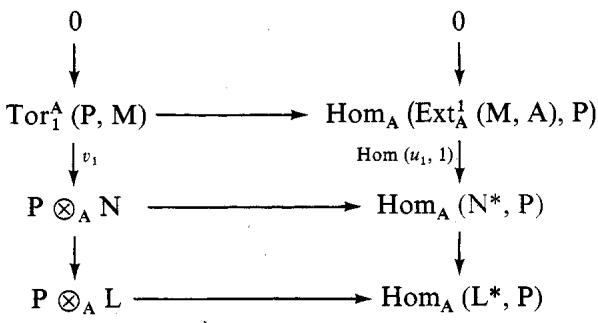
\includegraphics[keepaspectratio]{images/part001_66a54857.jpg}}

where the columns are exact; we deduce the result in this case. If \(n \geqslant 2\) , the maps \(u_n\) and \(v_n\) are bijective (X, p.~128, cor. 4 and p.~131, cor. 3). By the induction hypothesis, the canonical homomorphism

\[
\operatorname{Tor} _ {n - 1} ^ {\mathbf {A}} (\mathrm{P}, \mathrm{N}) \rightarrow \operatorname{Hom} _ {\mathbf {A}} \left(\operatorname{Ext} _ {\mathbf {A}} ^ {n - 1} (\mathrm{N}, \mathrm{A}), \mathrm{P}\right)
\]

is injective (resp. bijective); diagram (5) shows that the same holds for the canonical homomorphism \(\mathrm{Tor}_{n}^{\mathrm{A}}(\mathrm{P},\mathrm{M})\to \mathrm{Hom}_{\mathrm{A}}(\mathrm{Ext}_{\mathrm{A}}^{n}(\mathrm{M},\mathrm{A}),\mathrm{P})\) , which completes the proof.

\subsection{Homological dimension of a ring}

DEFINITION 2. --- One calls the homological dimension of A and denotes by dh(A) the least upper bound in \(\overline{\mathbf{Z}}\) of the set of integers \(n\) for which there exist two A-modules M and N such that \(\operatorname{Ext}_{\mathbf{A}}^{n}(\mathbf{M},\mathbf{N})\neq0\) .

One has \(\mathrm{dh}(0) = -\infty\) , \(\mathrm{dh(A)} \geqslant 0\) if \(A \neq 0\) . One will see below that \(\mathrm{dh(A)} = 1\) if \(A\) is principal and is not a field, and that, if \(K\) is a commutative field

\[
\mathrm{dh} (\mathrm{K} [ \mathrm{X} _ {1}, \dots , \mathrm{X} _ {n} ]) = n.
\]

PROPOSITION 4. --- Let n be an integer ≥ 0. The following conditions are equivalent: (i) dh(A) ≤ n,

\begin{enumerate}
\def\labelenumi{(\roman{enumi})}
\setcounter{enumi}{1}
\tightlist
\item
  for every A-module M, one has \(\mathrm{dp}_{\mathbf{A}}(\mathbf{M}) \leqslant n\) ,
\end{enumerate}

(ii') for every finitely generated A-module M, one has \(\mathrm{dp}_{\mathbf{A}}(\mathbf{M}) \leqslant n\) ,

\begin{enumerate}
\def\labelenumi{(\roman{enumi})}
\setcounter{enumi}{2}
\tightlist
\item
  for every exact sequence
\end{enumerate}

\[
0 \rightarrow \mathrm{K} \rightarrow \mathrm{P} _ {n - 1} \rightarrow \mathrm{P} _ {n - 2} \rightarrow \dots \rightarrow \mathrm{P} _ {0}
\]

where the \(P_{i}\) are projective, K is projective,

\begin{enumerate}
\def\labelenumi{(\roman{enumi})}
\setcounter{enumi}{3}
\tightlist
\item
  for every exact sequence
\end{enumerate}

\[
\mathrm{I} ^ {0} \rightarrow \mathrm{I} ^ {1} \rightarrow \dots \rightarrow \mathrm{I} ^ {n - 1} \rightarrow \mathrm{N} \rightarrow 0
\]

where the \(\mathrm{I}^{i}\) are injective, N is injective,

\begin{enumerate}
\def\labelenumi{(\alph{enumi})}
\setcounter{enumi}{21}
\tightlist
\item
  every A-module has an injective resolution of length ≤ n.
\end{enumerate}

The equivalence of conditions (i), (ii) and (iii) follows from prop. 1. We obviously have (ii) \(\Rightarrow\) (ii'). It therefore suffices for us to prove (ii') \(\Rightarrow\) (iv) \(\Rightarrow\) (v) \(\Rightarrow\) (i).

(ii') \(\Rightarrow\) (iv): with the notations of (iv), let K be the kernel of \(\mathrm{I}^{0} \to \mathrm{I}^{1}\) . By X, p.~128, cor. 4, we have for every A-module M an isomorphism \(\operatorname{Ext}_{\mathbf{A}}^{1}(\mathbf{M}, \mathbf{N}) \to \operatorname{Ext}_{\mathbf{A}}^{n+1}(\mathbf{M}, \mathbf{K})\) ; it then follows from (ii') that \(\operatorname{Ext}_{\mathbf{A}}^{1}(\mathbf{M}, \mathbf{N})\) is zero for every finitely generated A-module M. By X, p.~93, prop. 11, this implies that N is injective, whence (iv).

\begin{enumerate}
\def\labelenumi{(\roman{enumi})}
\setcounter{enumi}{3}
\tightlist
\item
  \(\Rightarrow\) (v): let M be an A-module. Applying (iv) to the exact sequence
\end{enumerate}

\[
0 \rightarrow \mathrm{M} \rightarrow \mathrm{I} ^ {0} (\mathrm{M}) \rightarrow \mathrm{I} ^ {1} (\mathrm{M}) \rightarrow \dots \rightarrow \mathrm{I} ^ {n - 1} (\mathrm{M}) \rightarrow \mathrm{K} ^ {n - 1} (\mathrm{M}) \rightarrow 0
\]

of X, p.~52, we conclude that \(\mathbf{K}^{n-1}(\mathbf{M})\) is injective, whence (v).

\begin{enumerate}
\def\labelenumi{(\alph{enumi})}
\setcounter{enumi}{21}
\tightlist
\item
  \(\Rightarrow\) (i): this follows from X, p.~100, th. 1.
\end{enumerate}

Remarks. --- 1) If \(\mathrm{dh}(\mathbf{A}) \leqslant n < +\infty\) , we have \(\operatorname{Tor}_{n+1}^{\mathbf{A}}(\mathbf{P}, \mathbf{M}) = 0\) for every A-module M and every right A-module P, since \(\mathrm{dp}_{\mathbf{A}}(\mathbf{M}) \leqslant n\) (cf.~lemma 1).

\begin{enumerate}
\def\labelenumi{\arabic{enumi})}
\setcounter{enumi}{1}
\tightlist
\item
  For dh(A) to be finite, it is necessary and sufficient that dp\_A(M) be finite for every nonzero A-module M. This indeed follows from what precedes and from X, p.~135, cor. 1.
\end{enumerate}

COROLLARY. --- Suppose A is left noetherian and let n be an integer \textgreater{} 0. The following conditions are equivalent:

\begin{enumerate}
\def\labelenumi{(\roman{enumi})}
\item
  \(\mathrm{dh(A)}\leqslant n,\)
\item
  for every pair of finitely generated A-modules M and N, we have \(\operatorname{Ext}_{\mathbf{A}}^{n+1}(\mathbf{M}, \mathbf{N}) = 0\) ,
\item
  for every finitely generated left A-module M and every finitely generated right A-module P, we have \(\operatorname{Tor}_{n+1}^{\mathbf{A}}(\mathbf{P},\mathbf{M}) = 0\) .
\end{enumerate}

This follows from props. 2 and 4.

Remark. --- By the equivalence of (i) and (iii), we have dh(A) = dh(A°) if A is right and left noetherian. This equality is not satisfied in general (X, p.~204, exercise 20).

PROPOSITION 5. --- Suppose A is left noetherian and of finite homological dimension and let \(\mathcal{C}_{0}\) (resp. \(\mathcal{C}\) ) be the set of isomorphism classes of finitely generated projective A-modules (resp. of finitely generated A-modules). Then the canonical homomorphism of Grothendieck groups \(\mathrm{K}(\mathcal{C}_{0}) \to \mathrm{K}(\mathcal{C})\) is bijective.

This follows from X, p.~137, cor.

\subsection{Rings of homological dimension 0}

PROPOSITION 6. --- The following conditions are equivalent:

\begin{enumerate}
\def\labelenumi{(\roman{enumi})}
\item
  every A-module is projective,
\item
  every A-module is injective,
\item
  every ideal of A is an injective module,
\item
  \(\mathrm{dh}(\mathbf{A})\leqslant 0,\)
\item
  A is semisimple,
\item
  A is noetherian and every A-module is flat,
\item
  every complex of A-modules is split,
\item
  every exact sequence of A-modules is split.
\end{enumerate}

By prop. 4, we have (i) \(\Leftrightarrow\) (ii) \(\Leftrightarrow\) (iv); by cor. 1 to prop. 4, we have (vi) \(\Rightarrow\) (iv). By X, p.~35, example 4, we have (i) \(\Rightarrow\) (vii); since (ii) \(\Rightarrow\) (iii) and (vii) \(\Rightarrow\) (viii) are trivial and since (viii) \(\Rightarrow\) (i) follows from II, p.~39, prop. 4, it remains to prove (iii) \(\Rightarrow\) (v) and (v) \(\Rightarrow\) (vi); the last assertion follows from VIII, § 5, no. 1, props. 1 and 2; finally, if every ideal of A is injective, it is a direct summand in A, whence (iii) \(\Rightarrow\) (v).

\subsection{Rings of homological dimension 1}

PROPOSITION 7. --- The following conditions are equivalent:

\begin{enumerate}
\def\labelenumi{(\roman{enumi})}
\item
  \(\mathrm{dh}(\mathbf{A})\leqslant 1\)
\item
  every submodule of a projective module is projective,
\end{enumerate}

(ii') every ideal of A is projective,

\begin{enumerate}
\def\labelenumi{(\roman{enumi})}
\setcounter{enumi}{2}
\item
  every quotient of an injective A-module is injective,
\item
  for every projective complex C, there exists a homologism \(\varphi : \mathbf{C} \to \mathbf{H}(\mathbf{C})\) such that \(\mathbf{H}(\varphi) = 1_{\mathbf{H}(\mathbf{C})}\) ,
\item
  for every injective complex C, there exists a homologism \(\psi : \mathrm{H}(\mathbf{C}) \to \mathbf{C}\) such that \(\mathrm{H}(\psi) = 1_{\mathrm{H}(\mathbf{C})}\) .
\item
  \(\Leftrightarrow\) (ii) \(\Leftrightarrow\) (iii): this follows from prop. 4 of X, p.~138.
\item
  \(\Rightarrow\) (iv): let C be a projective complex. If (ii) holds, the submodule B(C) of C is projective, whence (iv) by X, p.~35, remark b).
\item
  \(\Rightarrow\) (v): let C be an injective complex. If (iii) holds, the quotient \(B_{n}(C)\) of \(C_{n+1}\) is injective for every \(n\) , whence (v) by X, p.~35, remark a).
\item
  \(\Rightarrow\) (ii): let P be a projective A-module, M a submodule of P, \(i: \mathbf{M} \to \mathbf{P}\) the canonical injection. Let \(p: \mathbf{L} \to \mathbf{M}\) be a surjective homomorphism of a free module L onto M. Consider the projective complex C such that \(\mathbf{C}_1 = \mathbf{L}\) , \(\mathbf{C}_0 = \mathbf{P}\) , \(\mathbf{C}_i = 0\) for \(i \neq 0\) , \(1\) , \(d_1 = i \circ p\) . If (iv) is satisfied, let \(\varphi: \mathbf{C} \to \mathbf{H}(\mathbf{C})\) be a homologism such that \(\mathbf{H}(\varphi) = 1_{\mathbf{H}(\mathbf{C})}\) . Since \(\mathbf{H}_1(\mathbf{C}) = \operatorname{Ker} p\) , \(\varphi_1\) is a projector of L onto \(\operatorname{Ker} p\) , the exact sequence
\end{enumerate}

\[
0 \rightarrow \operatorname{Ker} p \rightarrow \mathrm{L} \xrightarrow {p} \mathrm{M} \rightarrow 0
\]

is split and M is isomorphic to a direct summand of L, hence is projective.

\begin{enumerate}
\def\labelenumi{(\alph{enumi})}
\setcounter{enumi}{21}
\tightlist
\item
  \(\Rightarrow\) (iii): let I be an injective module, M a quotient of I, \(\pi : \mathrm{I} \to \mathrm{M}\) the canonical projection. Let \(i: \mathrm{M} \to \mathrm{J}\) be an injective homomorphism of M into an injective module J. Consider the injective complex C such that \(C^0 = I\) , \(C^1 = J\) , \(C^i = 0\) for \(i \neq 0, 1\) , \(d^0 = i \circ \pi\) . If (v) is satisfied, let \(\psi : \mathrm{H}(\mathbf{C}) \to \mathbf{C}\) be a homologism such that \(\mathrm{H}(\psi) = 1_{\mathrm{H}(\mathbf{C})}\) . Since
\end{enumerate}

\[
\mathrm{H} ^ {1} (\mathrm{C}) = \text { Coker } i  ,
\]

\(\psi^{1}\) is a section of the canonical projection J → Coker i, and M is a direct summand in J, hence injective.

\begin{enumerate}
\def\labelenumi{(\roman{enumi})}
\setcounter{enumi}{1}
\tightlist
\item
  \(\Rightarrow\) (ii'): this is trivial.
\end{enumerate}

(ii') \(\Rightarrow\) (ii): this follows from VII, § 3, cor. 1 to th. 1.

Example. --- If A is principal, then dh(A) ≤ 1.

Remark. --- If A is (commutative) integral, the preceding conditions are also equivalent to the following:

Integral rings satisfying these conditions are called Dedekind rings (cf.~X, p.~204, exercise 12 and AC, VII, § 2, no. 2, th. 1).

COROLLARY. --- Let A be a ring of homological dimension ≤ 1, C a complex of projective A-modules, \(\tilde{C}\) a complex of projective right A-modules, C' a complex of injective A-modules, P a right A-module, M a left A-module, n an integer. We then have split exact sequences

\[
\begin{array}{r l} & 0 \to \bigoplus_ {p + q = n} \mathrm{H} _ {p} (\tilde {\mathrm{C}}) \otimes_ {\mathrm{A}} \mathrm{H} _ {q} (\mathrm{C}) \xrightarrow {\gamma} \mathrm{H} _ {n} (\tilde {\mathrm{C}} \otimes_ {\mathrm{A}} \mathrm{C}) \xrightarrow {\alpha} \bigoplus_ {p + q = n - 1} \mathrm{Tor} _ {1} ^ {\mathrm{A}} \left(\mathrm{H} _ {p} (\tilde {\mathrm{C}}), \mathrm{H} _ {q} (\mathrm{C})\right) \to 0, \\ & 0 \to \prod_ {p} \mathrm{Ext} _ {\mathrm{A}} ^ {1} \left(\mathrm{H} _ {p} (\mathrm{C}), \mathrm{H} ^ {n - p - 1} (\mathrm{C} ^ {\prime})\right) \xrightarrow {\beta} \mathrm{H} ^ {n} (\mathrm{Homgr} _ {\mathrm{A}} (\mathrm{C}, \mathrm{C} ^ {\prime})) \\ & \qquad \qquad \qquad \xrightarrow {\lambda_ {p}} \prod_ {p} \mathrm{Homgr} _ {\mathrm{A}} \left(\mathrm{H} _ {p} (\mathrm{C}), \mathrm{H} ^ {n - p} (\mathrm{C} ^ {\prime})\right) \to 0, \\ & 0 \to \mathrm{P} \otimes_ {\mathrm{A}} \mathrm{H} _ {n} (\mathrm{C}) \xrightarrow {\gamma_ {p}} \mathrm{H} _ {n} (\mathrm{P} \otimes_ {\mathrm{A}} \mathrm{C}) \xrightarrow {\alpha_ {p}} \mathrm{Tor} _ {1} ^ {\mathrm{A}} \left(\mathrm{P}, \mathrm{H} _ {n - 1} (\mathrm{C})\right) \to 0, \\ & 0 \to \mathrm{Ext} _ {\mathrm{A}} ^ {1} \left(\mathrm{H} _ {n - 1} (\mathrm{C}), \mathrm{M}\right) \xrightarrow {\beta_ {p}} \mathrm{H} ^ {n} (\mathrm{Homgr} _ {\mathrm{A}} (\mathrm{C}, \mathrm{M})) \xrightarrow {\lambda_ {p}} \mathrm{Hom} _ {\mathrm{A}} \left(\mathrm{H} _ {n} (\mathrm{C}), \mathrm{M}\right) \to 0. \end{array}
\]

Since \(Z(C)\) , \(B(C)\) , \(Z(\tilde{C})\) and \(B(\tilde{C})\) are projective and \(B(C')\) injective, this follows from \(X\) , p.~78, cor. 2, p.~96, cor. 1 and p.~98, cor. 2.

\subsection{Homological dimension of polynomial rings}

Lemma 2. --- Let \(\rho: \mathbf{A} \to \mathbf{A}'\) be a ring homomorphism, M an A-module, \(\mathbf{M}'\) a \(\mathbf{A}'\) -module. If the A-module \(\mathbf{A}_d'\) is flat, we have \(\mathrm{dp}_{\mathbf{A}'}(\mathbf{A}' \otimes_{\mathbf{A}} \mathbf{M}) \leqslant \mathrm{dp}_{\mathbf{A}}(\mathbf{M})\) . If the A-module \(\mathbf{A}_s'\) is projective, we have \(\mathrm{dp}_{\mathbf{A}}(\mathbf{M}') \leqslant \mathrm{dp}_{\mathbf{A}'}(\mathbf{M}')\) .

The first assertion is clear if \(\mathrm{dp}_{\mathbf{A}}(\mathbf{M}) = \pm \infty\) ; if \(\mathrm{dp}_{\mathbf{A}}(\mathbf{M}) = n \in \mathbb{N}\) , there exists an exact sequence of A-modules

\[
0 \rightarrow \mathrm{P} _ {n} \rightarrow \mathrm{P} _ {n - 1} \rightarrow \dots \rightarrow \mathrm{P} _ {0} \rightarrow \mathrm{M} \rightarrow 0
\]

where the \(P_{i}\) are projective; the sequence of A'-modules

\[
0 \rightarrow \mathrm{A} ^ {\prime} \otimes_ {\mathrm{A}} \mathrm{P} _ {n} \rightarrow \mathrm{A} ^ {\prime} \otimes_ {\mathrm{A}} \mathrm{P} _ {n - 1} \rightarrow \dots \rightarrow \mathrm{A} ^ {\prime} \otimes_ {\mathrm{A}} \mathrm{P} _ {0} \rightarrow \mathrm{A} ^ {\prime} \otimes_ {\mathrm{A}} \mathrm{M} \rightarrow 0
\]

is exact, since \(\mathbf{A}_d'\) is flat, and the \(\mathbf{A}'\) -modules \(\mathbf{A}' \otimes_{\mathbf{A}} \mathrm{P}_i\) are projective (II, p.~89, cor.); hence \(\mathrm{dp}_{\mathbf{A}'}(\mathbf{A}' \otimes_{\mathbf{A}} \mathbf{M}) \leqslant n = \mathrm{dp}_{\mathbf{A}}(\mathbf{M})\) . The second assertion is clear if \(\mathrm{dp}_{\mathbf{A}'}(\mathbf{M}') = \pm \infty\) ; if \(\mathrm{dp}_{\mathbf{A}'}(\mathbf{M}') = m \in \mathbf{N}\) , there exists an exact sequence of \(\mathbf{A}'\) -modules

\[
0 \to \mathrm{P} _ {m} ^ {\prime} \to \mathrm{P} _ {m - 1} ^ {\prime} \to \dots \to \mathrm{P} _ {0} ^ {\prime} \to \mathrm{M} ^ {\prime} \to 0,
\]

where the \(P_{i}^{\prime}\) are projective; the sequence of underlying A-modules is exact. On the other hand, each \(P_{i}^{\prime}\) is a direct summand of an A'-submodule of a module \(A_{s}^{\prime(I)}\) , hence is a projective A-module; we therefore have \(\mathrm{dp}_{\mathbf{A}}(\mathbf{M}^{\prime}) \leqslant m = \mathrm{dp}_{\mathbf{A}^{\prime}}(\mathbf{M}^{\prime})\) .

Lemma 3. --- Suppose A is commutative and let M be an A{[}X{]}-module.

\begin{enumerate}
\def\labelenumi{\alph{enumi})}
\item
  We have \(\mathrm{dp}_{\mathbf{A}}(\mathbf{M}) \leqslant \mathrm{dp}_{\mathbf{A}[\mathbf{X}]}(\mathbf{M}) \leqslant \mathrm{dp}_{\mathbf{A}}(\mathbf{M}) + 1\) .
\item
  If the homothety \(X_{M}\) is injective, we have dp \(_{A}\) (M/XM) ≤ dp \(_{A[X]}\) (M).
\item
  If \(\mathbf{XM} = 0\) , we have \(\mathrm{dp}_{\mathbf{A}}(\mathbf{M}) + 1 = \mathrm{dp}_{\mathbf{A}[\mathbf{X}]}(\mathbf{M}).\)
\item
  We have an exact sequence of A{[}X{]}-modules (III, p.~106 and VII, § 5, no. 1)
\end{enumerate}

\[
0 \rightarrow \mathrm{A} [ \mathrm{X} ] \otimes_ {\mathrm{A}} \mathrm{M} \rightarrow \mathrm{A} [ \mathrm{X} ] \otimes_ {\mathrm{A}} \mathrm{M} \rightarrow \mathrm{M} \rightarrow 0;
\]

Assertion (a) then follows from X, p.~135, cor. 2 and from Lemma 2.

\begin{enumerate}
\def\labelenumi{\alph{enumi})}
\setcounter{enumi}{1}
\tightlist
\item
  If \(\mathrm{dp}_{\mathbf{A}[\mathbf{X}]}(\mathbf{M}) = \pm \infty\) the assertion is trivial. If \(\mathbf{M}\) is projective and nonzero, then the A-module \(\mathbf{M} / \mathbf{XM}\) is identified with \(\mathbf{A} \otimes_{\mathbf{A}[\mathbf{X}]} \mathbf{M}\) , hence is projective, and we have \(\mathrm{dp}_{\mathbf{A}}(\mathbf{M} / \mathbf{XM}) \leqslant 0 = \mathrm{dp}_{\mathbf{A}[\mathbf{X}]}(\mathbf{M})\) . Let us reason by induction on \(\mathrm{dp}_{\mathbf{A}[\mathbf{X}]}(\mathbf{M}) = n\) , assumed \(>0\) . Consider an exact sequence of \(\mathbf{A}[\mathbf{X}]\) -modules \(0 \to \mathbf{N} \to \mathbf{L} \to \mathbf{M} \to 0\) , where \(\mathbf{L}\) is a free \(\mathbf{A}[\mathbf{X}]\) -module; applying to the diagram
\end{enumerate}

\[
\begin{array}{c} 0 \longrightarrow \mathrm{N} \longrightarrow \mathrm{L} \longrightarrow \mathrm{M} \longrightarrow 0 \\ \mathrm {X_ {N}} \Big \downarrow \quad \mathrm {X_ {L}} \Big \downarrow \quad \mathrm {X_ {M}} \Big \downarrow \\ 0 \longrightarrow \mathrm{N} \longrightarrow \mathrm{L} \longrightarrow \mathrm{M} \longrightarrow 0 \end{array}
\]

prop. 2 of X, p.~4, we see that \(X_{N}\) is injective and that we have the exact sequence

\[
0 \rightarrow \mathrm{N} / \mathrm{XN} \rightarrow \mathrm{L} / \mathrm{XL} \rightarrow \mathrm{M} / \mathrm{XM} \rightarrow 0.
\]

Since L is free over A{[}X{]}, L/XL is free over A and we have

\[
\mathrm{dp} _ {\mathbf {A} [ \mathbf {X} ]} (\mathbf {N}) = n - 1, \quad \mathrm{dp} _ {\mathbf {A}} (\mathbf {M} / \mathbf {X M}) \leqslant 1 + \mathrm{dp} _ {\mathbf {A}} (\mathbf {N} / \mathbf {X N});
\]

as dp \(_{A}\) (N/XN) ≤ n - 1 by the induction hypothesis, we deduce dp \(_{A}\) (M/XM) ≤ n, which is what had to be proved.

\begin{enumerate}
\def\labelenumi{\alph{enumi})}
\setcounter{enumi}{2}
\tightlist
\item
  The assertion is trivial if \(\mathrm{dp}_{\mathbf{A}[\mathbf{X}]}(\mathbf{M}) = \pm \infty\) , and also if \(\mathrm{dp}_{\mathbf{A}[\mathbf{X}]}(\mathbf{M}) = 0\) (which is impossible since \(\mathbf{XM} = 0\) ). We may therefore assume \(\mathrm{dp}_{\mathbf{A}[\mathbf{X}]}(\mathbf{M}) = n > 0\) . Considering as above an exact sequence \(0 \to \mathbf{N} \to \mathbf{L} \to \mathbf{M} \to 0\) , where \(\mathbf{L}\) is a free \(\mathbf{A}[\mathbf{X}]\) -module, we obtain an exact sequence of \(\mathbf{A}\) -modules
\end{enumerate}

\[
0 \rightarrow \mathrm{M} \rightarrow \mathrm{N} / \mathrm{XN} \rightarrow \mathrm{L} / \mathrm{XL} \rightarrow \mathrm{M} \rightarrow 0.
\]

By b), we have \(\mathrm{dp}_{\mathbf{A}}(\mathbf{N} / \mathbf{X}\mathbf{N}) \leqslant \mathrm{dp}_{\mathbf{A}[\mathbf{X}]}(\mathbf{N}) = \mathrm{dp}_{\mathbf{A}[\mathbf{X}]}(\mathbf{M}) - 1 = n - 1\) ; since \(\mathrm{dp}_{\mathbf{A}}(\mathbf{L} / \mathbf{XL}) = 0\) , we deduce from the preceding exact sequence, applying X, p.~135, cor. 2 twice, that \(\mathrm{dp}_{\mathbf{A}}(\mathbf{M}) \leqslant n - 1\) . But, by a), we have

\[
\mathrm{dp} _ {\mathbf {A}} (\mathbf {M}) \geqslant \mathrm{dp} _ {\mathbf {A} [ \mathbf {X} ]} (\mathbf {M}) - 1 = n - 1,
\]

whence c).

THEOREM 1. --- Suppose A is commutative. Then

\[
\mathrm{dh} (\mathbf {A} [ \mathbf {X} ]) = \mathrm{dh} (\mathbf {A}) + 1.
\]

For every A{[}X{]}-module M, we have (lemma 3)

\[
\mathrm{dp} _ {\mathbf {A} [ \mathbf {X} ]} (\mathbf {M}) \leqslant \mathrm{dp} _ {\mathbf {A}} (\mathbf {M}) + 1 \leqslant \mathrm{dh} (\mathbf {A}) + 1
\]

hence \(\mathrm{dh}(\mathbf{A}[\mathbf{X}]) \leqslant \mathrm{dh}(\mathbf{A}) + 1\) ; conversely, if \(\mathbf{M}\) is an A-module, let \(\overline{\mathbf{M}}\) be the \(\mathbf{A}[\mathbf{X}]\) -module obtained by endowing \(\mathbf{M}\) with the structure for which \(\mathbf{X}\mathbf{M} = 0\) , then (lemma 3)

\[
\mathrm{d} p _ {\mathrm{A}} (\mathrm{M}) = \mathrm{d} p _ {\mathrm{A} [ \mathrm{X} ]} (\overline {{\mathrm{M}}}) - 1 \leqslant \mathrm{d} h (\mathrm{A} [ \mathrm{X} ]) - 1,
\]

hence dh(A) ≤ dh(A{[}X{]}) - 1.

COROLLARY 1. --- Suppose A is commutative. We have

\[
\mathrm{dh} (\mathrm{A} [ \mathrm{X} _ {1}, \dots , \mathrm{X} _ {n} ]) = \mathrm{dh} (\mathrm{A}) + n.
\]

This follows from the theorem by induction on n.

COROLLARY 2. --- Let K be a commutative field (resp. a principal ideal ring * or a Dedekind ring * which is not a field). Then dh(K{[}X₁, \ldots, Xₙ{]}) is equal to n (resp. n + 1). This follows from the fact that dh(K) = 0 (resp. dh(K) = 1).

\subsection{Homological dimension of graded modules}

In this section, we assume that A is a graded ring with degrees ≥ 0. We denote by \((\mathbf{A}_{n})_{n \in \mathbf{Z}}\) its grading; we thus have \(A_{n} = 0\) for n \textless{} 0, \(A_{0}\) is a subring of A, \(J_{0} = \bigoplus_{n > 0} A_{n}\) is a two-sided ideal of A and the quotient graded ring \(A/J_{0}\) is identified with \(A_{0}\) .

Lemma 4. --- Let M be a graded A-module bounded below (X, p.~56). If \(\mathbf{A}_0\otimes_{\mathbf{A}}\mathbf{M} = 0\) , then \(\mathbf{M} = 0\) .

Since \(A_{0} \otimes_{A} M\) is isomorphic to \(M/J_{0} M\) , this is none other than II, p.~171, prop. 6.

Lemma 5. --- Let M be a graded A-module bounded below, and let

\[
s: \mathbf {A} \otimes_ {\mathbf {A} _ {0}} \mathrm{M} / \mathrm{J} _ {0} \mathrm{M} \rightarrow \mathrm{M}
\]

be a graded A-homomorphism such that \(1 \otimes_{\mathbf{A}} s: \mathbf{A}_0 \otimes_{\mathbf{A}} (\mathbf{A} \otimes_{\mathbf{A}_0} \mathbf{M} / \mathrm{J}_0 \mathbf{M}) \to \mathbf{A}_0 \otimes_{\mathbf{A}} \mathbf{M}\) is the canonical isomorphism. Then s is surjective. If \(\operatorname{Tor}_1^{\mathbf{A}}(\mathbf{A}_0, \mathbf{M}) = 0\) , s is bijective.

We have an exact sequence

\[
0 \rightarrow \operatorname{Ker} s \rightarrow A \otimes_ {A _ {0}} M / J _ {0} M \xrightarrow {s} M \rightarrow \operatorname{Coker} s \rightarrow 0
\]

and the graded A-modules Ker \(s\) and Coker \(s\) are bounded below. From the exact sequence \(\mathbf{A}_{0} \otimes_{\mathbf{A}} (\mathbf{A} \otimes_{\mathbf{A}_{0}} \mathrm{M} / \mathrm{J}_{0} \mathrm{M}) \xrightarrow{1 \otimes s} \mathbf{A}_{0} \otimes_{\mathbf{A}} \mathrm{M} \to \mathbf{A}_{0} \otimes_{\mathbf{A}} \text{Coker } s \to 0\) , we deduce that \(\mathbf{A}_{0} \otimes_{\mathbf{A}} \text{Coker } s = 0\) , hence \(s\) is surjective (lemma 4). We then have an exact sequence

\[
\operatorname{Tor} _ {1} ^ {\mathrm{A}} \left(\mathrm{A} _ {0}, \mathrm{M}\right)\rightarrow \mathrm{A} _ {0} \otimes_ {\mathrm{A}} \operatorname{Ker} s \rightarrow \mathrm{A} _ {0} \otimes_ {\mathrm{A}} \left(\mathrm{A} \otimes_ {\mathrm{A} _ {0}} \mathrm{M} / \mathrm{J} _ {0} \mathrm{M}\right) \xrightarrow {1 \otimes s} \mathrm{A} _ {0} \otimes_ {\mathrm{A}} \mathrm{M}.
\]

If \(\operatorname{Tor}_1^{\mathbf{A}}(\mathbf{A}_0, \mathbf{M}) = 0\) , then \(\mathbf{A}_0 \otimes_{\mathbf{A}} \operatorname{Ker} s = 0\) and \(s\) is injective (lemma 4).

PROPOSITION 8. --- Let M be a graded A-module bounded below.

\begin{enumerate}
\def\labelenumi{\alph{enumi})}
\tightlist
\item
  The following conditions are equivalent:
\end{enumerate}

\begin{enumerate}
\def\labelenumi{(\roman{enumi})}
\item
  M is isomorphic to a graded A-module of the form \(\mathbf{A} \otimes_{\mathbf{A}_0} \mathbf{N}\) , where \(N\) is a graded projective (resp. graded free) \(\mathbf{A}_0\) -module;
\item
  M is a projective (resp. free) graded A-module;
\item
  \(\mathbf{M} / \mathbf{J}_0\mathbf{M}\) is a projective (resp. graded free) \(\mathbf{A}_0\) -module and \(\operatorname{Tor}_1^{\mathbf{A}}(\mathbf{A}_0,\mathbf{M}) = 0\) .
\end{enumerate}

\begin{enumerate}
\def\labelenumi{\alph{enumi})}
\setcounter{enumi}{1}
\tightlist
\item
  Suppose moreover that M has a generating system consisting of homogeneous elements of bounded degrees. Then the following conditions are equivalent:
\end{enumerate}

\begin{enumerate}
\def\labelenumi{(\roman{enumi})}
\item
  The graded A-module M possesses a finite composition series whose quotients are isomorphic to graded A-modules of the form \(A \otimes_{A_{0}} N\) , where N is a flat graded \(A_{0}\) -module;
\item
  M is a flat A-module;
\item
  \(\mathbf{M} / \mathrm{J}_0\mathbf{M}\) is a flat \(\mathbf{A}_0\) -module and \(\operatorname{Tor}_1^{\mathbf{A}}(\mathbf{A}_0,\mathbf{M}) = 0\) .
\end{enumerate}

In each of the two cases, we evidently have (i) \(\Rightarrow\) (ii) \(\Rightarrow\) (iii). We must therefore prove (iii). \(\Rightarrow\) (i).

\begin{enumerate}
\def\labelenumi{\alph{enumi})}
\tightlist
\item
  The graded A-module A \(\otimes_{\mathbf{A}_0}\mathbf{M} / \mathbf{J}_0\) M is a projective A-module since \(\mathbf{M} / \mathbf{J}_0\) M is a projective \(\mathbf{A}_0\) -module. The canonical homomorphism of A-modules
\end{enumerate}

\[
p: \mathbf {M} \rightarrow \mathbf {M} / \mathrm{J} _ {0} \mathbf {M}
\]

is surjective; there therefore exists a graded A-homomorphism of degree zero

\[
s: \mathbf {A} \otimes_ {\mathbf {A} _ {0}} \mathbf {M} / \mathrm{J} _ {0} \mathbf {M} \rightarrow \mathbf {M}
\]

such that \(p \circ s(a \otimes x) = ax\) for \(a \in A\) and \(x \in M / J_0 M\) .

By Lemma 5, \(s\) is an isomorphism of A-modules from \(\mathbf{A} \otimes_{\mathbf{A}_0} \mathrm{M} / \mathrm{J}_0 \mathrm{M}\) over \(\mathbf{M}\) , whence (i).

\begin{enumerate}
\def\labelenumi{\alph{enumi})}
\setcounter{enumi}{1}
\tightlist
\item
  By the hypothesis on M, there exist integers a, b such that \(a \leqslant b\) such that M is generated by \(\oplus M_{i}\) Let us reason by induction on the positive integer b - a.
\end{enumerate}

If \(b - a = 0\) then M is generated by \(\mathbf{M}_a\) and the canonical \(\mathbf{A}_0\) -homomorphism \(\mathbf{M}_a \to \mathbf{M} / \mathbf{J}_0\) M is bijective; one then deduces from the A-homomorphism \(\mathbf{A} \otimes_{\mathbf{A}_0} \mathbf{M}_a \to \mathbf{M}\) defined by the structure of M as an A-module a graded A-homomorphism

\[
s: \mathbf {A} \otimes_ {\mathbf {A} _ {0}} \mathbf {M} / \mathrm{J} _ {0} \mathbf {M} \rightarrow \mathbf {M}
\]

satisfying the condition of Lemma 5. Then, by Lemma 5, s is bijective, whence (i).

In the general case, let \(\mathbf{M}^{(a)}\) be the (graded) sub-A-module of M generated by \(M_{a}\) and \(M'\) the quotient \(\mathbf{M}/\mathbf{M}^{(a)}\) . We have an exact sequence

\[
0 \to \mathbf {M} ^ {(a)} \xrightarrow {f} \mathbf {M} \xrightarrow {g} \mathbf {M} ^ {\prime} \to 0,
\]

whence, since \(\mathrm{Tor}_{1}^{\mathbf{A}}(\mathbf{A}_{0},\mathbf{M}) = 0\) by hypothesis, exact sequences

\begin{enumerate}
\def\labelenumi{(\arabic{enumi})}
\setcounter{enumi}{5}
\tightlist
\item
\end{enumerate}

\[
\begin{array}{c} \operatorname{Tor} _ {2} ^ {\mathsf {A}} (\mathbf {A} _ {0}, \mathbf {M} ^ {\prime}) \to \operatorname{Tor} _ {1} ^ {\mathsf {A}} (\mathbf {A} _ {0}, \mathbf {M} ^ {(a)}) \to 0 \\ 0 \to \operatorname{Tor} _ {1} ^ {\mathsf {A}} (\mathbf {A} _ {0}, \mathbf {M} ^ {\prime}) \to \operatorname{M} ^ {(a)} / \mathrm{J} _ {0} \operatorname{M} ^ {(a)} \xrightarrow {1 \otimes f} \operatorname{M} / \mathrm{J} _ {0} \operatorname{M} \xrightarrow {1 \otimes g} \operatorname{M} ^ {\prime} / \mathrm{J} _ {0} \operatorname{M} ^ {\prime} \to 0. \end{array}\tag{7}
\]

But the canonical homomorphism \(M_{a} \to M^{(a)}/J_{0} M^{(a)}\) is bijective. It follows that the homomorphism \(1 \otimes f : M^{(a)}/J_{0} M^{(a)} \to M/J_{0} M\) is injective and that its image is a sub- \(A_{0}\) -module direct summand of \(M/J_{0} M\) . It then follows from the exact sequence (7) that \(\operatorname{Tor}_{1}^{A}(A_{0}, M') = 0\) and that the \(A_{0}\) -module \(M'/J_{0} M'\) is flat since it is isomorphic to a direct summand of \(M/J_{0} M\) . By the induction hypothesis (which applies to \(M'\) since the latter is generated by the \(M'^{i}\) for \(a < i \leqslant b\) ), \(M'\) satisfies condition (i), hence is flat. One then deduces from the exact sequence (6) that \(\operatorname{Tor}_{1}^{A}(A_{0}, M^{(a)}) = 0\) , but \(M^{(a)}/J_{0} M^{(a)}\) is identified with \(M_{a}\) which is a flat \(A_{0}\) -module (as a direct summand submodule of \(M/J_{0} M\) ); by what has already been proved, the graded A-module \(M^{(a)}\) is isomorphic to \(A \otimes_{A_{0}} M_{a}\) hence also satisfies (i), which completes the proof.

COROLLARY 1. --- Let M be a finitely generated graded A-module. If the \(\mathbf{A}_0\) -module \(\mathrm{M} / \mathrm{J}_0\) M is projective (resp. graded free, resp. flat) and if \(\operatorname{Tor}_1^{\mathbf{A}}(\mathbf{A}_0, \mathbf{M}) = 0\) then the A-module M is projective (resp. graded free, resp. flat).

Corollary 2. --- Suppose that every projective \(\mathbf{A}_{0}\) -module is free (resp. that A be noetherian and that every finitely generated projective \(\mathbf{A}_{0}\) -module be free). Let M be a graded A-module bounded below (resp. a finitely generated graded A-module) and let n be an integer \(\geqslant 0\) such that \(\mathrm{dp}_{\mathbf{A}}(\mathbf{M}) \leqslant n\) . There exists an exact sequence of graded A-modules and graded homomorphisms of degree 0

\[
0 \rightarrow \mathrm{L} _ {n} \rightarrow \mathrm{L} _ {n - 1} \rightarrow \dots \rightarrow \mathrm{L} _ {0} \rightarrow \mathrm{M} \rightarrow 0
\]

where the \(L_{i}\) are graded free and bounded below (resp. graded free and finitely generated).

Indeed, there exists (X, p.~56, prop. 11) an exact sequence of graded A-modules and homomorphisms of degree 0

\[
0 \to \mathrm{L} _ {n} \to \mathrm{L} _ {n - 1} \to \dots \to \mathrm{L} _ {0} \to \mathrm{M} \to 0
\]

where the \(L_{i}\) are bounded below (resp. finitely generated) for \(0 \leqslant i \leqslant n\) and graded free for \(0 \leqslant i \leqslant n - 1\) .

Since \(\mathrm{dp}_{\mathbf{A}}(\mathbf{M}) \leqslant n\) the A-module \(L_{n}\) is projective; therefore \(\mathbf{A}_0 \otimes_{\mathbf{A}} L_n\) is a projective \(\mathbf{A}_0\) -module, hence graded free; since \(L_{n}\) is bounded below and \(\mathbf{A}_0 \otimes_{\mathbf{A}} L_n\) graded free, \(L_{n}\) is graded free (prop. 7).

COROLLARY 3 (Hilbert's syzygy theorem). --- Suppose that \(\mathbf{A}_0\) is a commutative field and that A is generated as \(\mathbf{A}_0\) -algebra by \(n\) homogeneous elements of degrees \(>0\) algebraically independent. For every graded A-module M bounded below (resp. of finite type), there exists an exact sequence of graded A-modules and graded homomorphisms of degree 0

\[
0 \rightarrow L _ {n} \rightarrow L _ {n - 1} \rightarrow \dots \rightarrow L _ {0} \rightarrow M \rightarrow 0,
\]

where the \(L_{i}\) are graded free and bounded below (resp. and finitely generated).

Indeed, \(\mathrm{dh}(\mathbf{A}) = n\) by theorem 1 of X, p.~143, and one applies cor. 2.

Remark. --- Cor. 2 also applies to the following cases:

\begin{enumerate}
\def\labelenumi{\alph{enumi})}
\item
  \(\mathbf{A}_0\) is principal and \(\mathbf{A} = \mathbf{A}_0[\mathbf{X}_1, \dots, \mathbf{X}_{n-1}]\) ;
\item
  * A \(_{0}\) is a regular local noetherian ring of dimension r and A = A \(_{0}\) {[}X \(_{1}\) , \ldots, X \(_{n}\) , r{]}. *
\end{enumerate}

COROLLARY 4. --- Assume \(\mathbf{A}_{0}\) semisimple. Let M be a graded A-module bounded below and n an integer \(\geqslant 0\) . For \(\mathrm{dp}_{\mathbf{A}}(\mathbf{M}) \leqslant n\) , it is necessary and sufficient that \(\operatorname{Tor}_{n+1}^{\mathbf{A}}(\mathbf{A}_{0}, \mathbf{M}) = 0\) .

If \(\mathrm{dp}_{\mathbf{A}}(\mathbf{M}) \leqslant n\) , then \(\operatorname{Tor}_{n+1}^{\mathbf{A}}(\mathbf{A}_0, \mathbf{M}) = 0\) (X, p.~135, lemma 1). Conversely, let \(0 \to \mathbf{K} \to \mathbf{L}_{n-1} \to \ldots \to \mathbf{L}_1 \to \mathbf{L}_0 \to \mathbf{M} \to 0\) be an exact sequence of graded A-modules bounded below such that \(\mathbf{L}_0, \ldots, \mathbf{L}_{n-1}\) are graded free (X, p.~56, prop. 11); by cor. 3 of X, p.~131, the equality \(\operatorname{Tor}_{n+1}^{\mathbf{A}}(\mathbf{A}_0, \mathbf{M}) = 0\) implies \(\operatorname{Tor}_1^{\mathbf{A}}(\mathbf{A}_0, \mathbf{K}) = 0\) ; since \(\mathbf{K} / \mathbf{J}_0\mathbf{K}\) is a projective \(\mathbf{A}_0\) -module since \(\mathbf{A}_0\) is semisimple (X, p.~140, prop. 6), K is projective by prop. 8 (X, p.~144), and \(\mathrm{dp}_{\mathbf{A}}(\mathbf{M}) \leqslant n\) .

COROLLARY 5. --- Suppose the ring \(\mathbf{A}_0\) semisimple. If \(\operatorname{Tor}_{n+1}^{\mathbf{A}}(\mathbf{A}_0, \mathbf{A}_0) = 0\) , we have \(\mathrm{dp}_{\mathbf{A}}(\mathbf{M}) \leqslant n\) for every graded \(\mathbf{A}\) -module bounded below.

Let A° denote the opposite graded ring of A: we have (A°)₀ = (A₀)°, so (A°)₀ is semisimple (VIII, § 5, n° 1, remark 3). Since \(\operatorname{Tor}_{n+1}^{A°}(A₀°, A₀°) = 0\) , we have \(\mathrm{dp}_A(A₀s) \leqslant n\) by Cor. 4: this implies \(\operatorname{Tor}_{n+1}^{A°}(M₀, A₀°) = 0\) for every A-module M, hence \(\operatorname{Tor}_{n+1}^{A}(A₀, M) = 0\) and we apply Cor. 4.

\section{KOSZUL COMPLEXES}

In this paragraph, all rings considered are commutative.
